\documentclass[assd_tp3_main.tex]{subfiles}
\begin{document}

\subsection{Implementación}

Para realizar la implementación práctica, se utilizó de base el circuito propuesto en las indicaciones del trabajo práctico, realizando las modificaciones pertinentes para su correcto funcionamiento. El diagrama en bloques del circuito es el siguiente.

\begin{figure}[!ht]
\begin{centering}
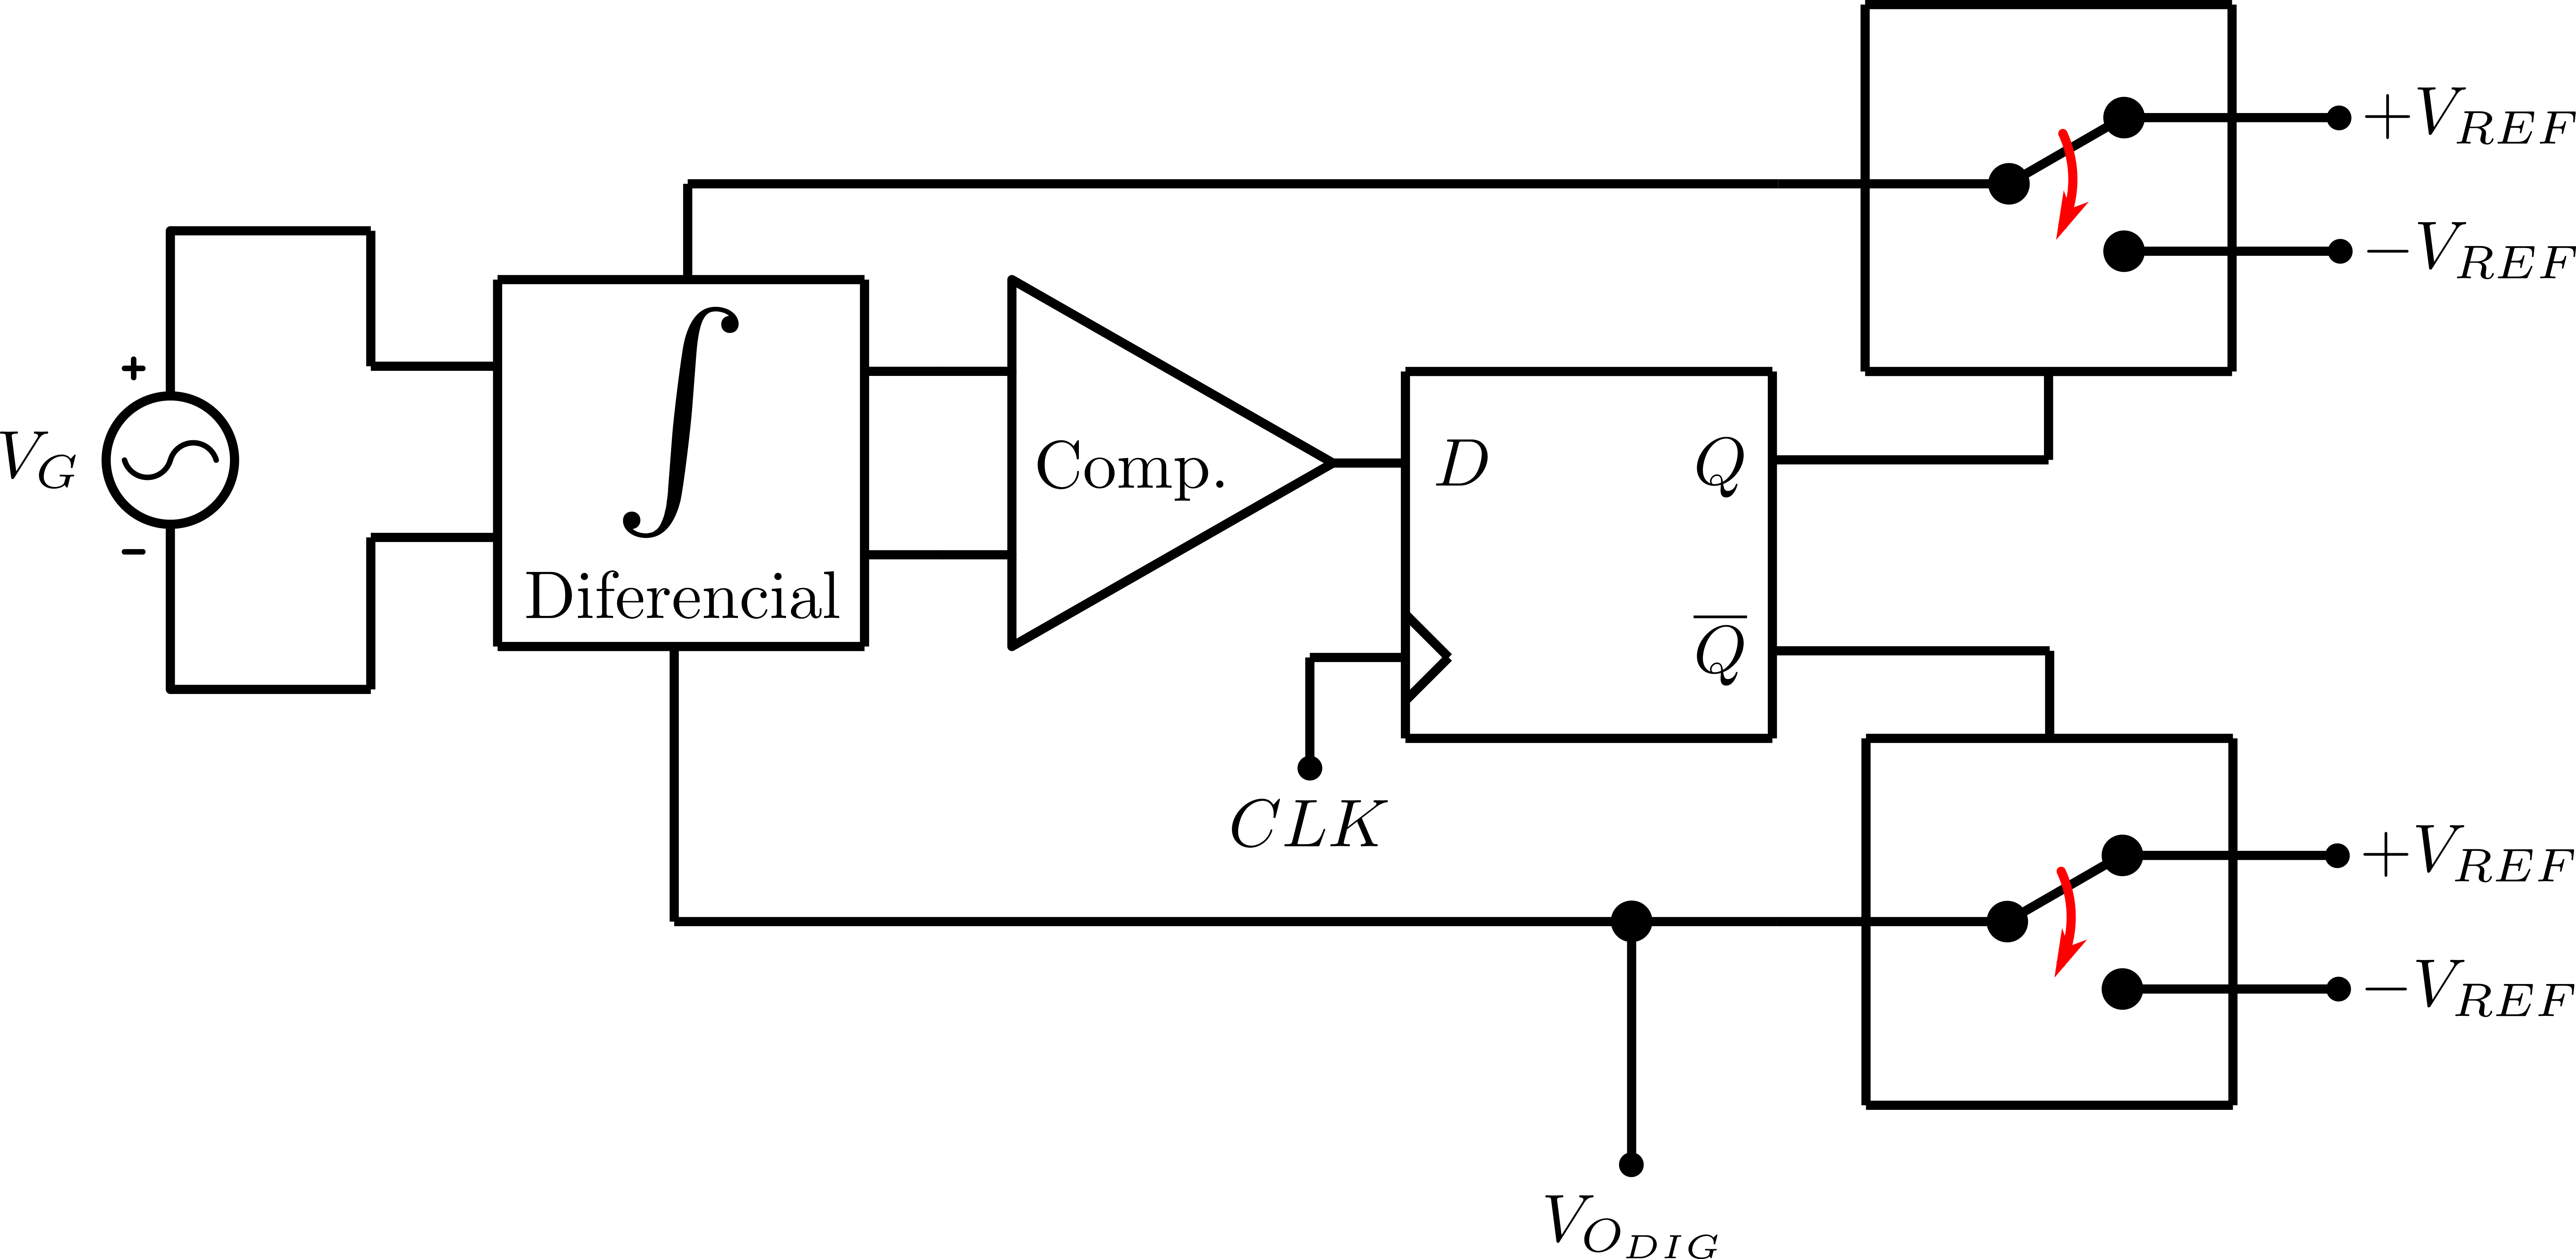
\includegraphics[scale=0.5]{images/ej5/Diagrama.png}
\par\end{centering}
\caption{Diagrama en bloques}
\end{figure}

\subsubsection{Oscilador}

Para implementar el oscilador, se utilizó el VCO integrado en el PLL CD4046. Partiendo de los extremos teóricos pedidos:

\[
f_{MIN} = 60KHz \hspace{2cm} f_{MAX} = 1MHz
\]

Se calcula el cociente entre ambos:

\[
\frac{f_{MAX}}{f_{MIN}} = 16.\hat{6}
\] 

Tomando la hoja de datos de Texas Instruments, a partir del gráfico de $\frac{f_{MAX}}{f_{MIN}}$, se obtiene la relación $\frac{R_2}{R_1}$:

\begin{figure}[!ht]
\begin{centering}
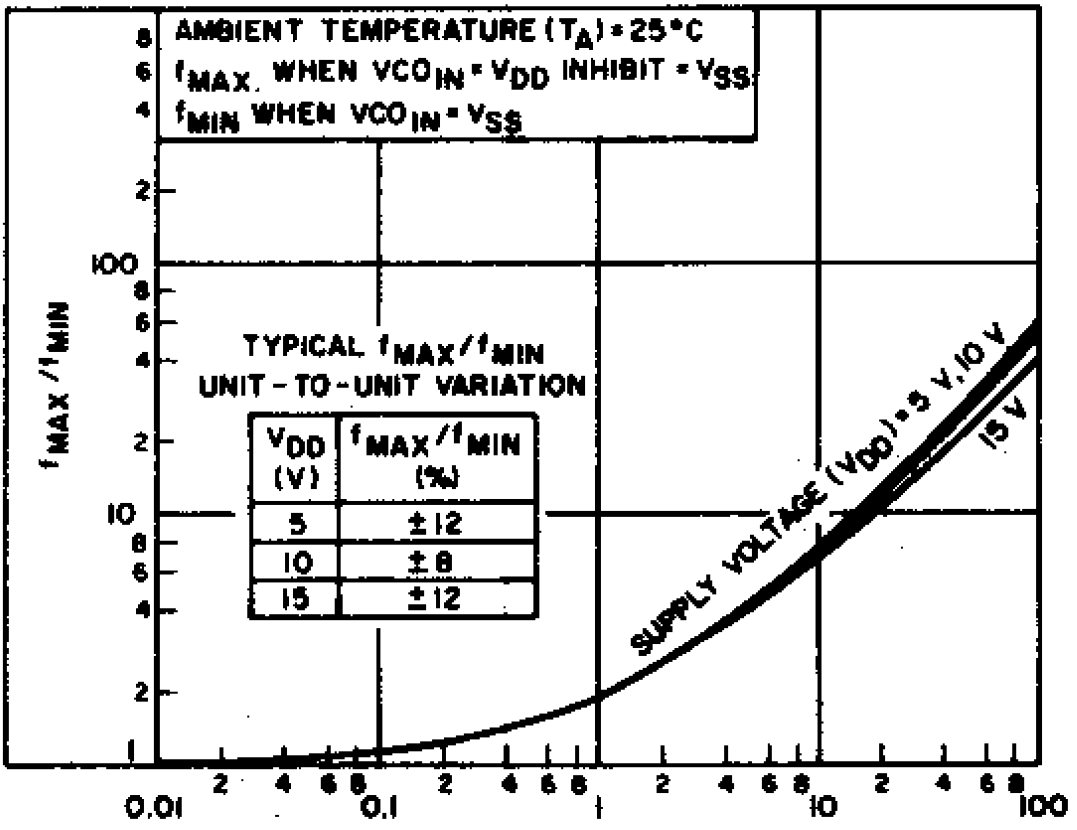
\includegraphics[scale=0.4]{images/ej5/f2f1.png}
\par\end{centering}
\caption{Gráfica del cociente entre las frecuencias en función de la relación de resistencias}
\end{figure}

De donde se obtiene que la relación es aproximadamente 40. Para una $R_2(N) = 680K\Omega$, resulta $R_1(N) = 18K\Omega$.
\newpage
De la gráfica de rectas de $R_2$ en función de $C_1$:

\begin{figure}[!ht]
\begin{centering}
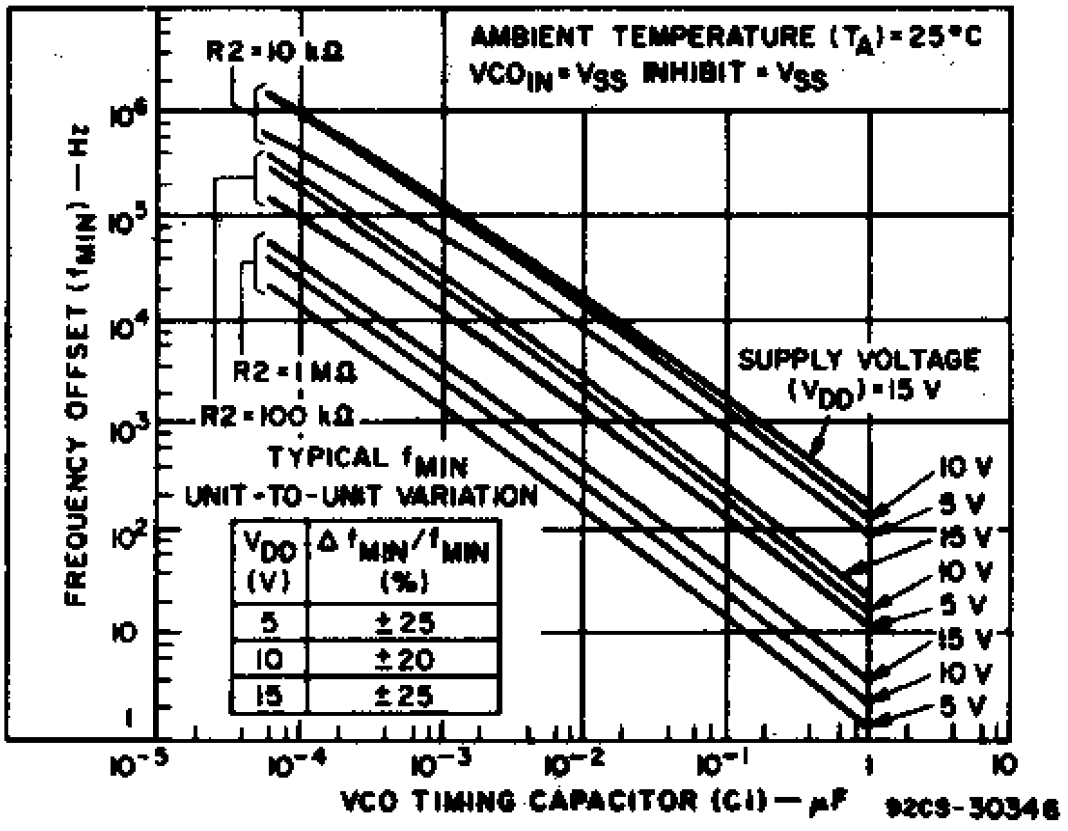
\includegraphics[scale=0.4]{images/ej5/r2c1.png}
\par\end{centering}
\caption{Gráfica de rectas de $R_2$ para valores de $C_1$}
\end{figure}

Se obtiene un valor aproximado de $C_1(N) = 39pF$. Dada la alta dispersión que posee el circuito para el cociente de las frecuencias, se ajusto el valor de $R_1$ en el PCB a $R_1(N) = 4.7K$, logrando finalmente un intervalo de frecuencias práctico de entre 52KHz a 1.14MHz. En las figuras siguientes se muestran ambas señales obtenidas correspondientes a los extremos.

\begin{figure}[!ht]
\begin{centering}
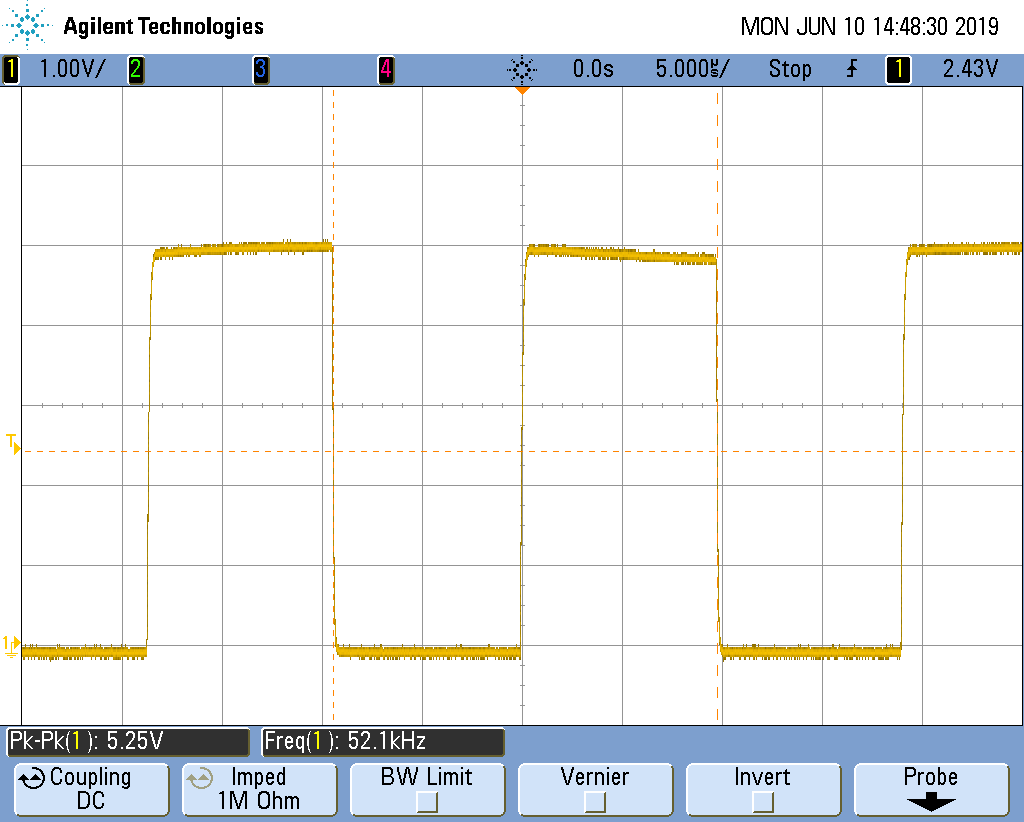
\includegraphics[scale=0.2]{../EJ4/Mediciones/Clk/clk_min.png}
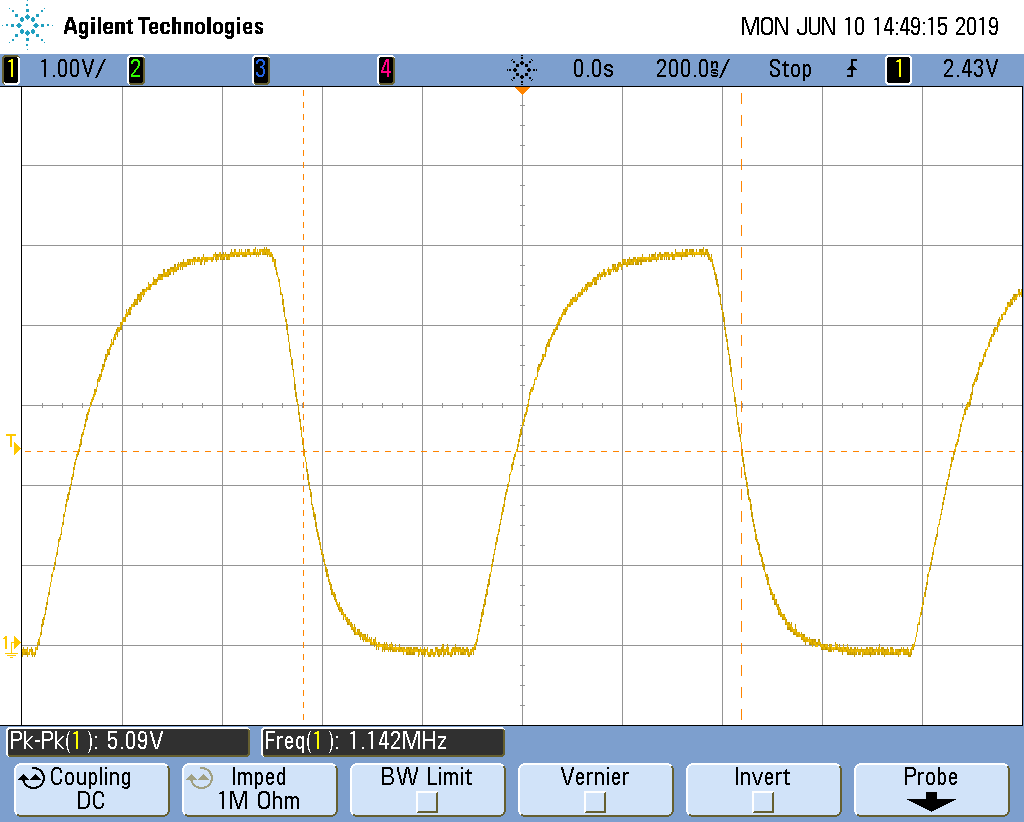
\includegraphics[scale=0.2]{../EJ4/Mediciones/Clk/clk_max.png}
\par\end{centering}
\caption{Gráfica de rectas de $R_2$ para valores de $C_1$}
\end{figure}

\subsubsection{Filtros Antialiasing - Recuperador}

El objetivo para el diseño de ambos filtros es que resulten de bajo orden, aprovechando la ventaja de estar realizando oversamplig, lo cual sitúa las repeticiones del espectro de la señal de entrada considerablemente separados.\par
Para elegir la frecuencia de corte de los filtros, se considera como limitación a la mínima frecuencia de sampleo que provee el clock diseñado anteriormente. El peor caso de ancho de banda de entrada se da con la señal 1/2 Gauss, dado que su discontinuidad tipo escalón produce una gran cantidad de armónicos. Esta señal se puede modelar como una señal cuadrada multiplicada por una gaussiana que se repite con el mismo período. Visto desde la frecuencia, resulta la convolución del espectro de la señal cuadrada (el cual ya conocemos que es muy grande) con el de la gaussiana, el cual tiene también forma de gaussiana. Dado que ambas señales son periódicas, sus espectros son discretos, por lo que se puede pensar que el espectro de la señal gaussiana se monta en cada una de las deltas del espectro de la señal cuadrada, por lo que el espectro de la señal resultante (1/2 Gauss en el tiempo) sigue siendo tan grande como el de la señal cuadrada.\par
Teniendo esto en cuenta, para tratar de incluir la mayor cantidad de armónicos posibles sin obtener aliasing a la salida, se ubicó la frecuencia de corte una década antes de la $f_{MIN}$ del clock, es decir $f_c = 6$KHz. Utilizando un filtro de orden 2, se logra para la frecuencia de 60KHz (es decir, donde se encontraría la primer repetición en el peor caso) una atenuación de 40dB. Dado que para las señales de prueba se pide que sean de una frecuencia mínima, se perderán varios armónicos para el caso de 1/2 Gauss, como se mostrará en las mediciones.\par
Teniendo el orden del filtro (2), por simplicidad se implementa utilizando dos integradores compensados en cascada, como se muestra en la figura.

\begin{figure}[!ht]
\begin{centering}
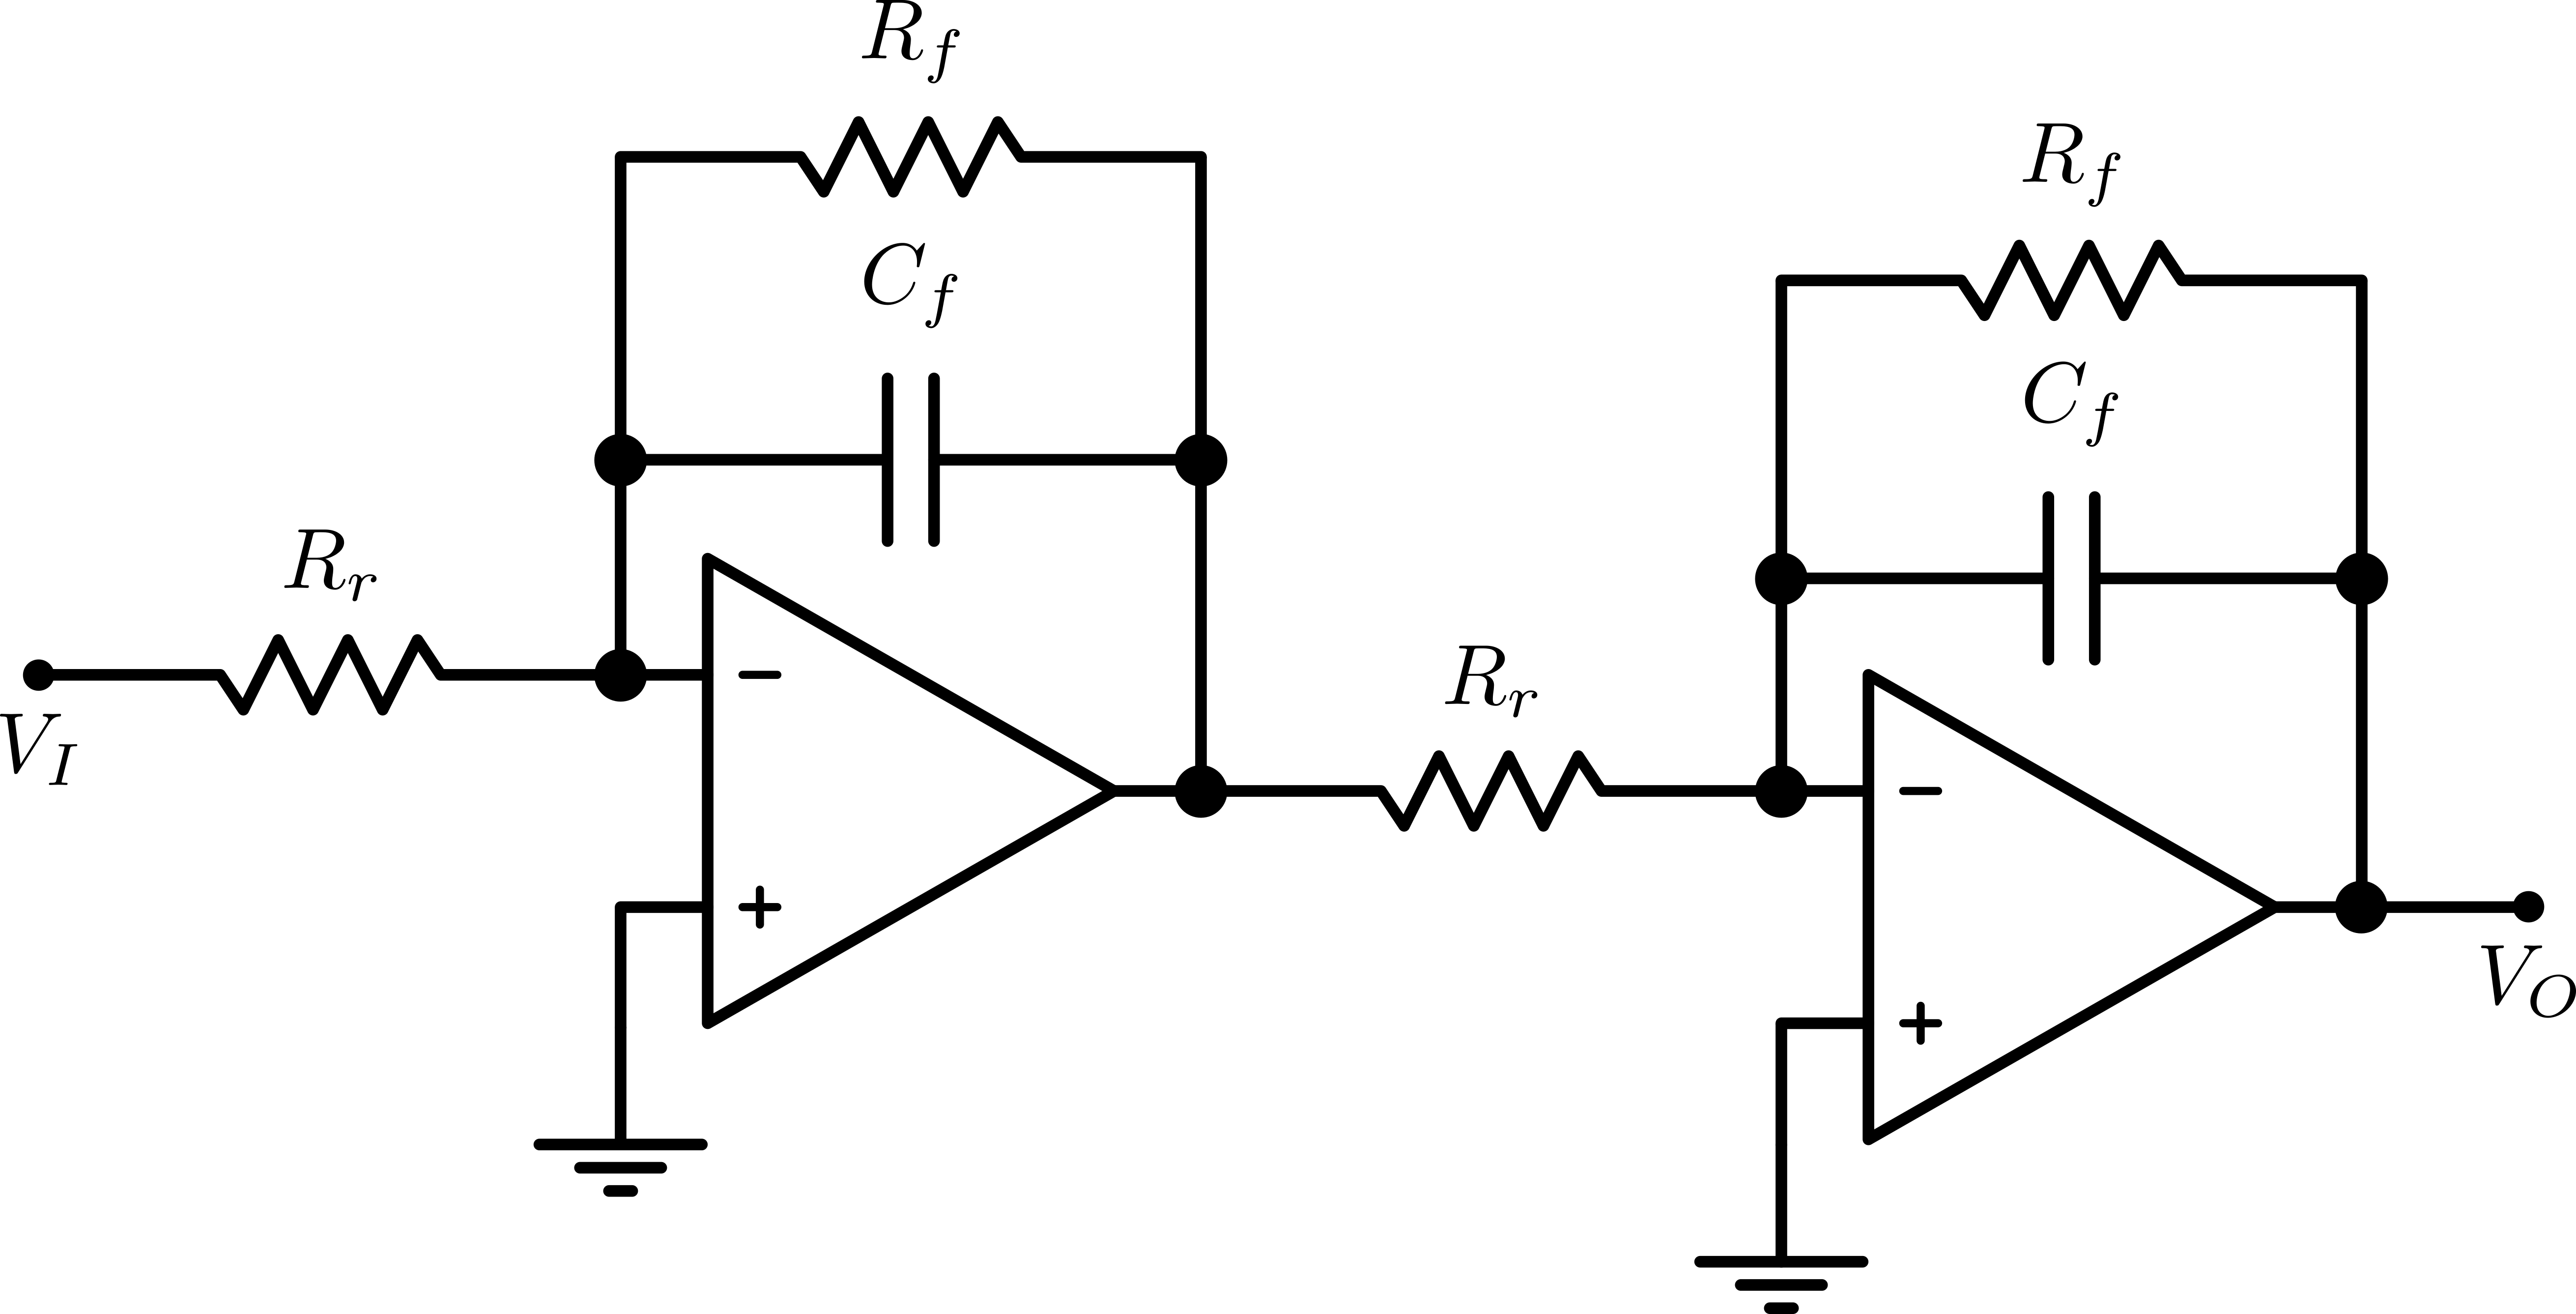
\includegraphics[scale=0.45]{images/ej5/Filtro.png}
\par\end{centering}
\caption{Filtro de orden 2 con integradores compensados}
\end{figure}

La transferencia de cada uno, usando la expresión conocida para un amplificador no inversor:

\[
A_V = -\frac{Z_f}{Z_r} = -\frac{R_f}{R_i(1+sC_fR_f)}
\]

Donde la frecuencia de corte:

\[
f_c = \frac{1}{2 \pi R_f C_f}
\]

Teniendo en cuenta la frecuencia de corte $f_c = 6$KHz, proponiendo $C_f = 10nF$, se despeja $R_f$:

\[
R_f = \frac{1}{2 \pi f_c C_f} = 2.65K\Omega \Longrightarrow R_f(N) = 2.7K\Omega
\] 

Dado que en banda pasante el filtro debe tener ganancia unitaria, se define también $R_i(N) = R_f(N) = 2.7K\Omega$

\subsubsection{Diferenciador}

En la implementación propuesta, el modulador posee entrada diferencial (en lugar de una sola entrada referida a masa). Esto permite cancelar bastante el ruido en modo común, lo cual resulta como una ventaja adicional dado que se trabajará con frecuencias de clock de hasta 1MHz, y éste podría provocar interferencias en la señal muestreada con capacitores switcheados de manera no deseada si no se toman algunas consideraciones en el layout del PCB (que se explicará luego). El circuito diferenciador se implementó con amplificadores operacionales, como se muestra a continuación.

\begin{figure}[!ht]
\begin{centering}
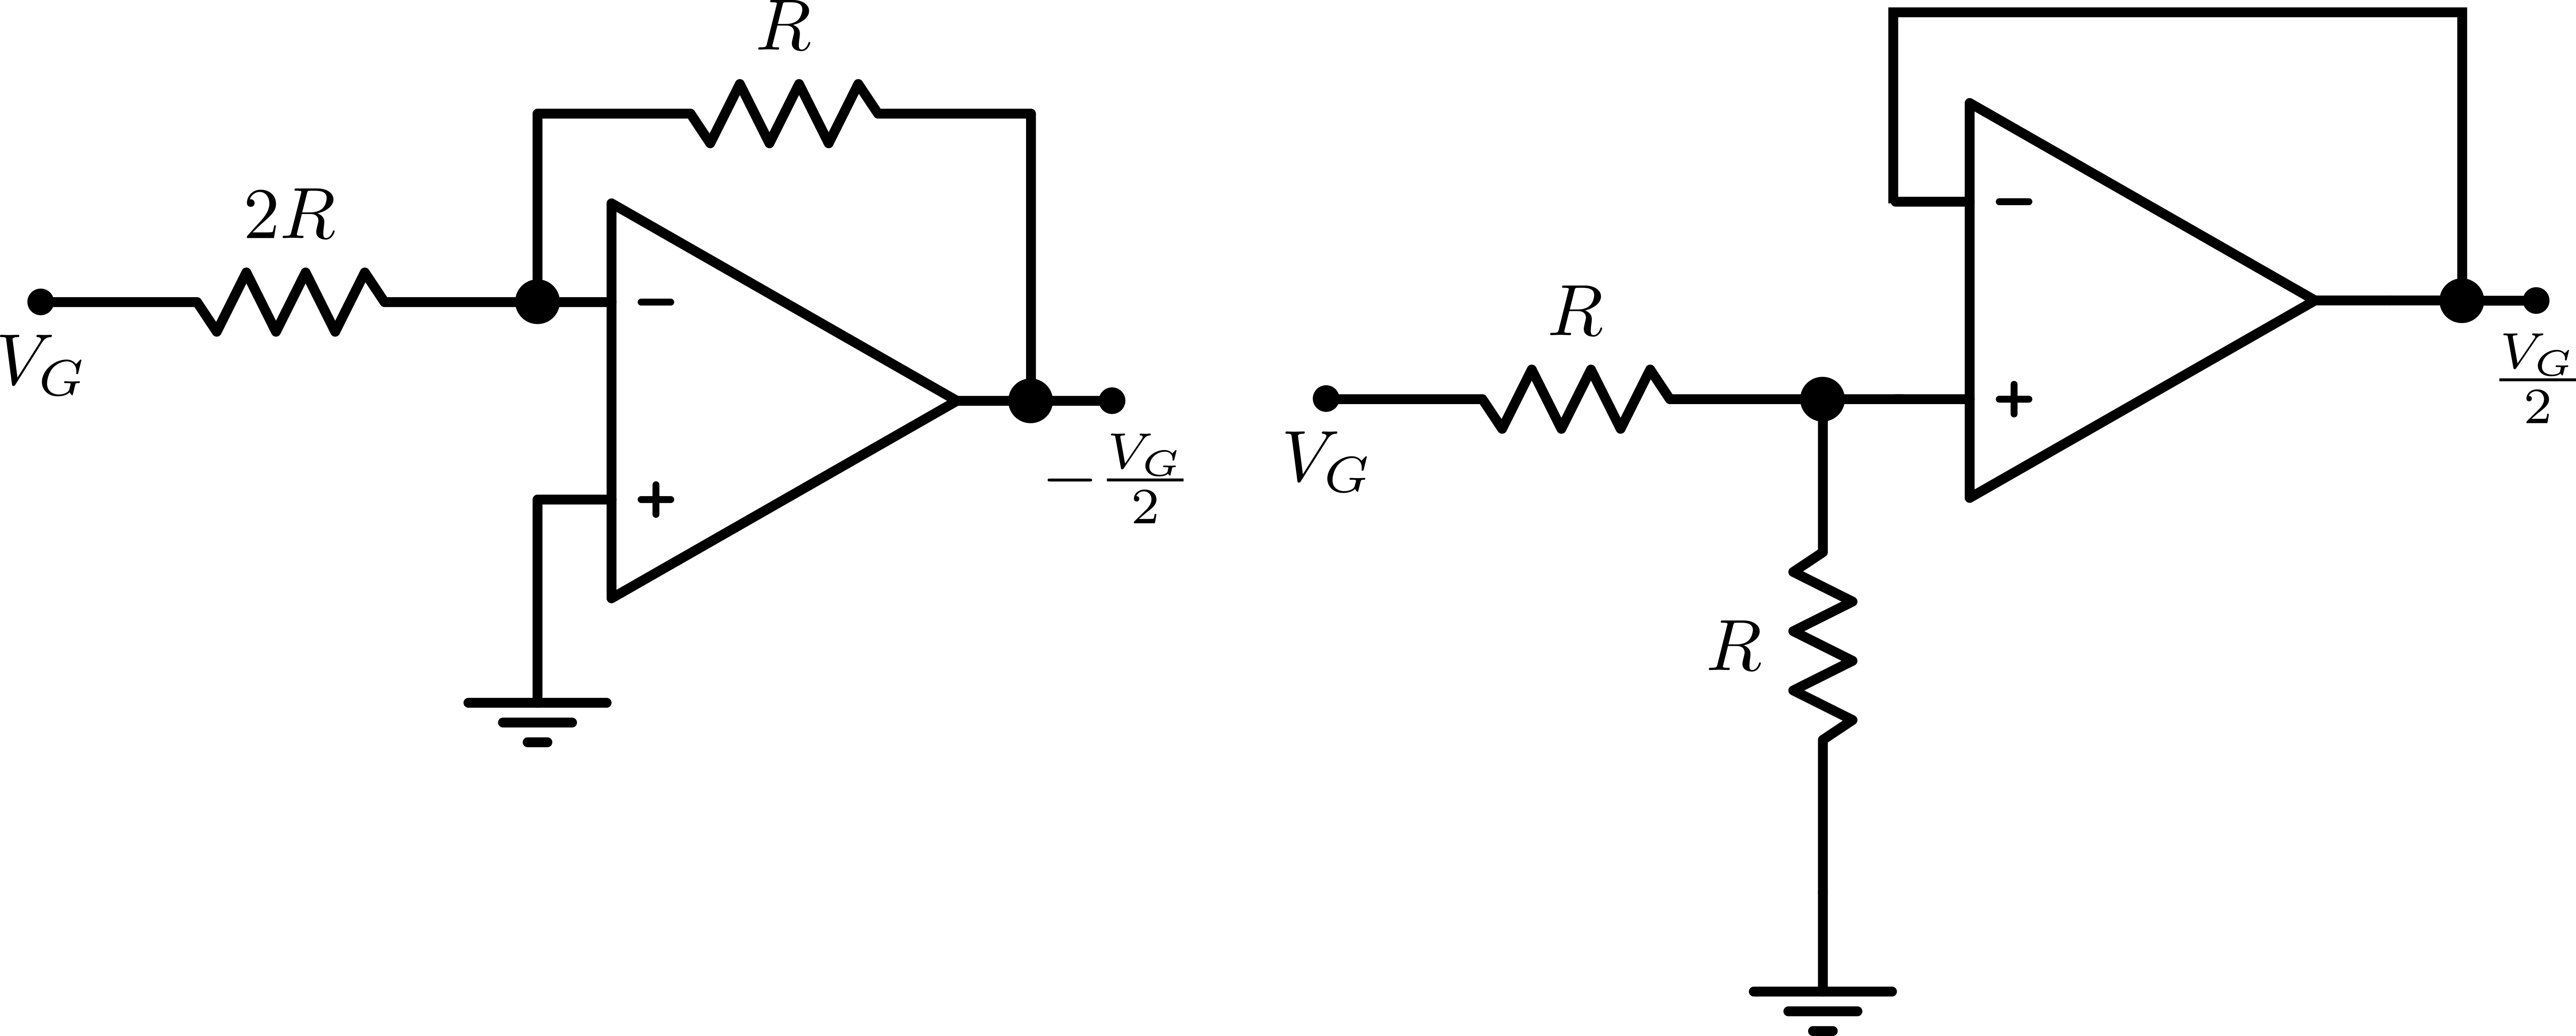
\includegraphics[scale=0.45]{images/ej5/diferenciador.png}
\par\end{centering}
\caption{Generador de señal diferencial}
\end{figure}

\subsubsection{Integrador con switched capacitors (SC)}

La idea se basa en la conmutación de los terminales del capacitor entre tensiones diferentes, que para el análisis deben ser suficientemente estables durante el tiempo T que dura la conmutación. Dicha conmutación suele realizarse con llaves simuladas mediante transistores MOS, pero para simplificar la comprensión se lo esquematiza con llaves ideales, como se muestra a continuación.

\begin{figure}[!ht]
\begin{centering}
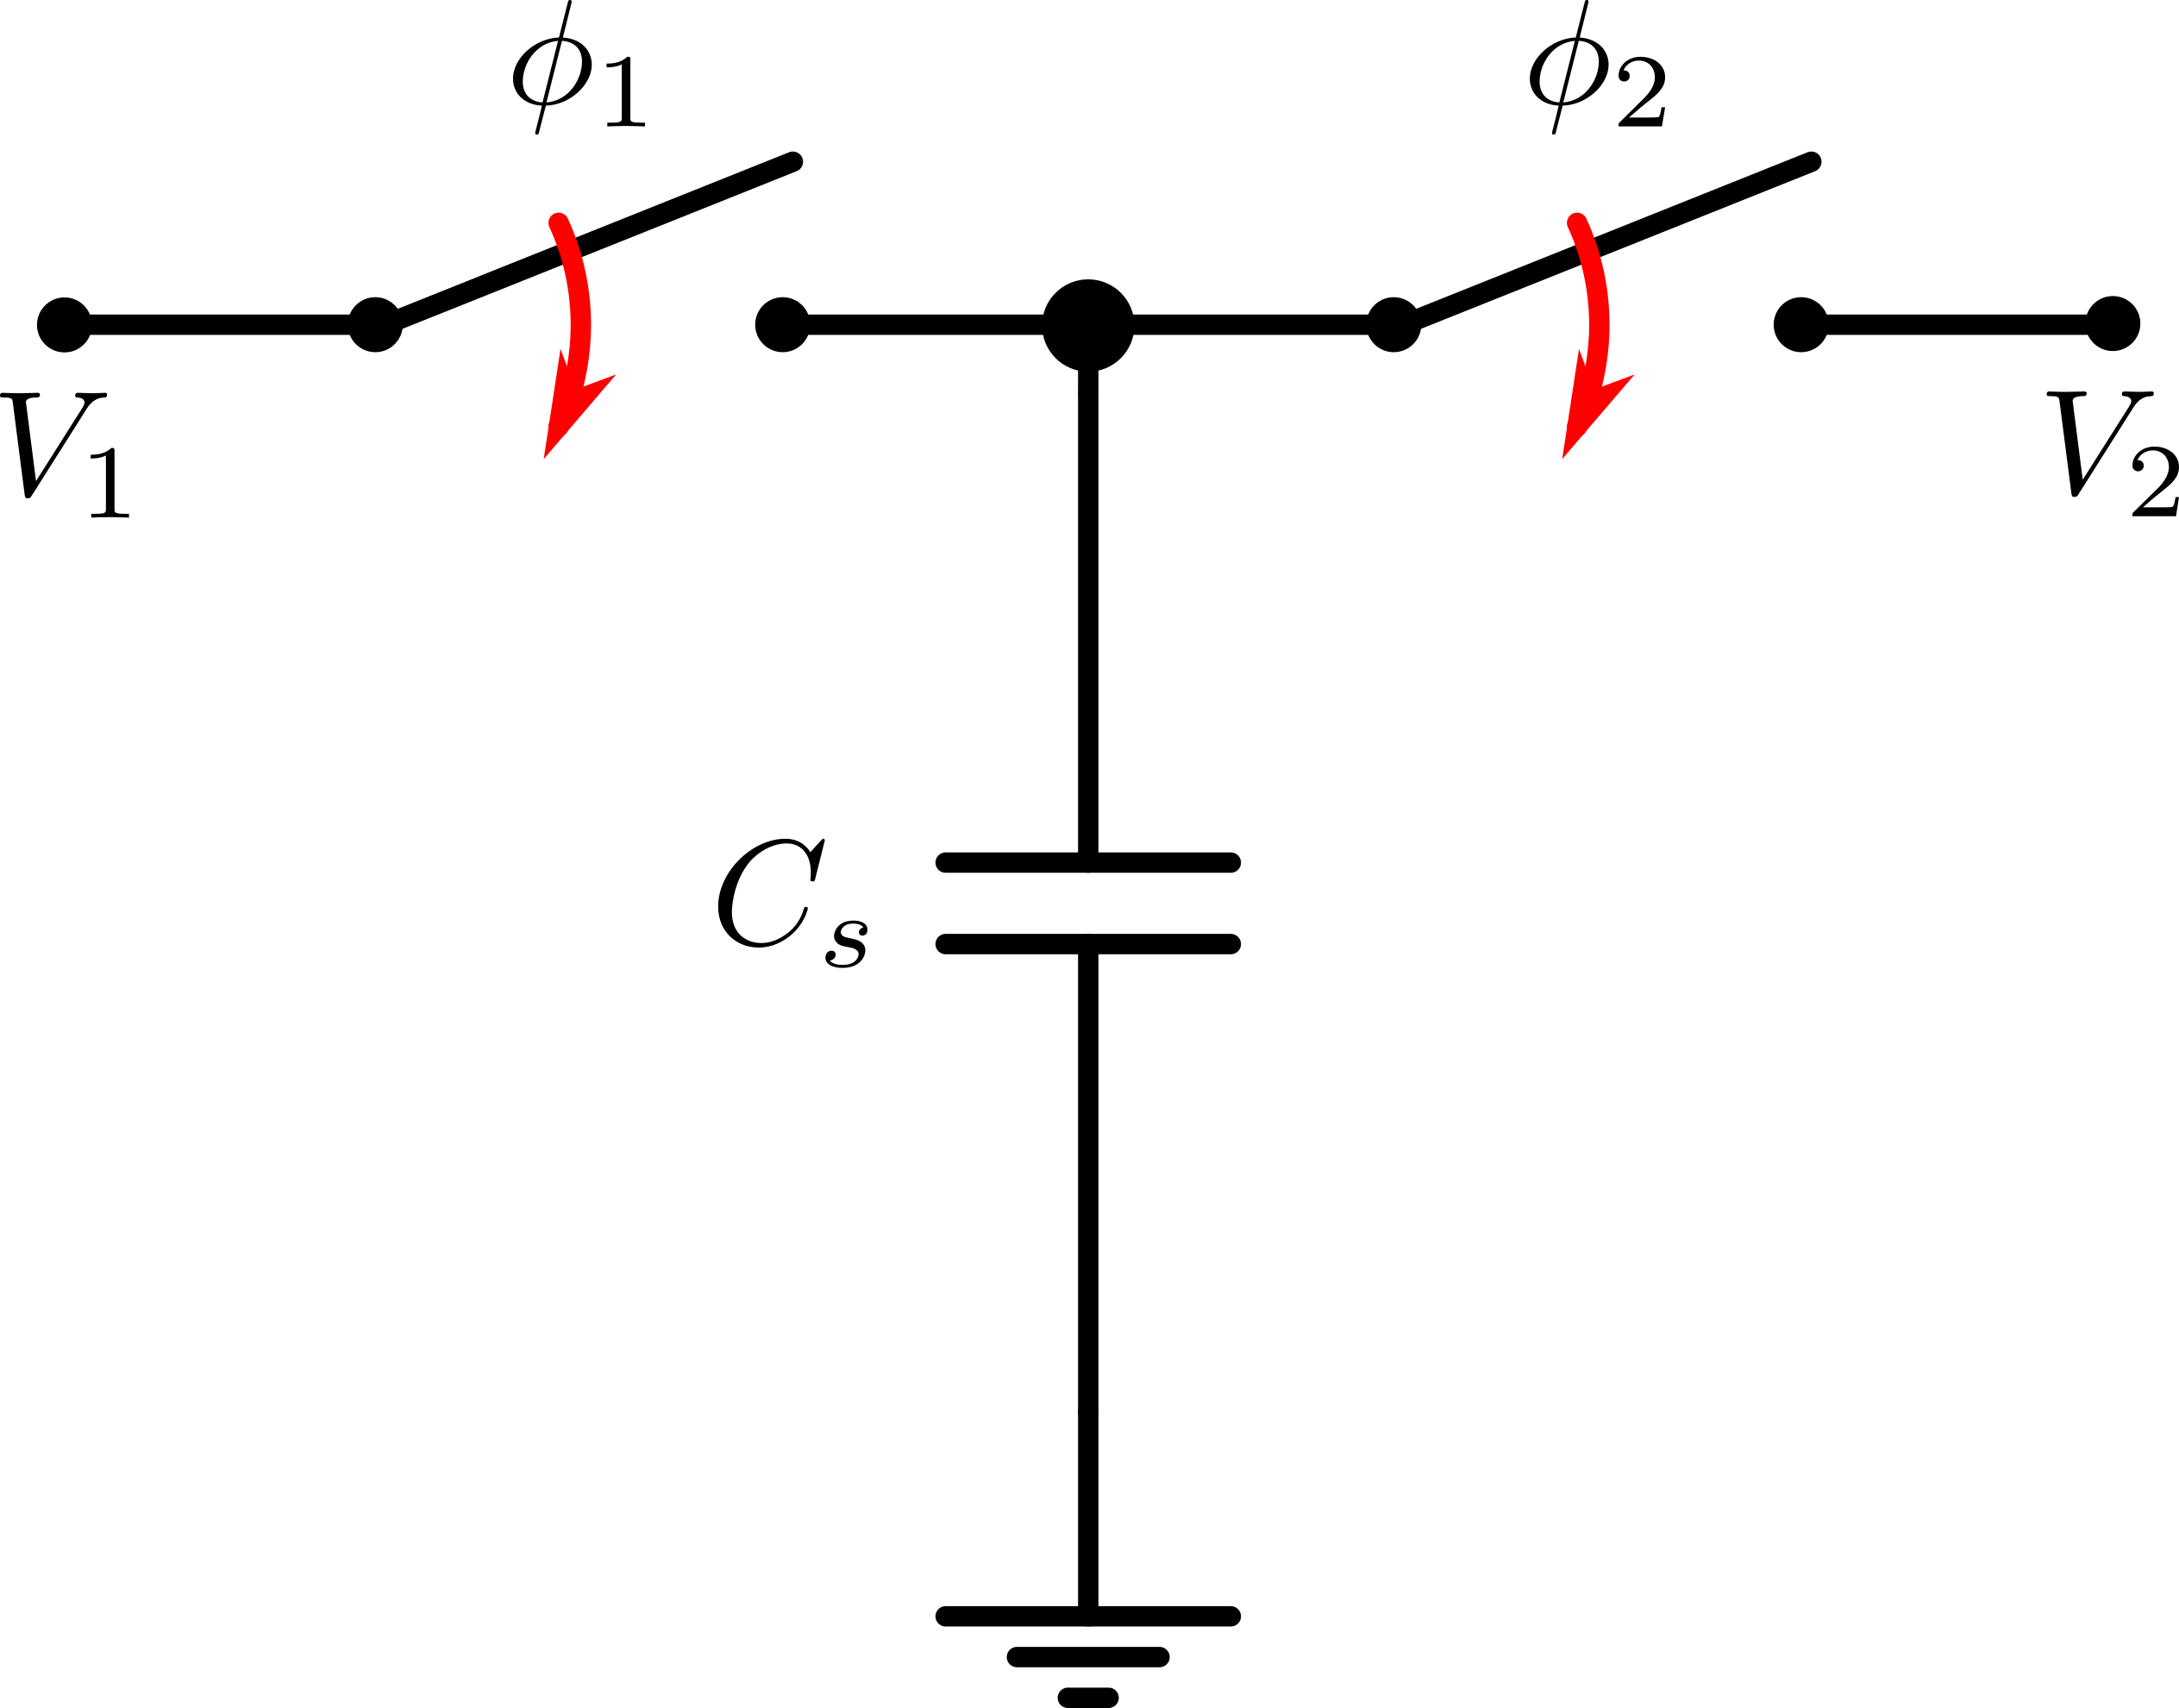
\includegraphics[scale=0.5]{images/ej5/SCBasico.png}
\par\end{centering}
\caption{Esquema de capacitor switcheado}
\end{figure}

Supongase que inicialmente se tiene al capacitor cargado con la tensión $V_2$, con ambos switches abiertos. Luego, se cierrra el switch $\phi_1$, conectando ahora el terminal del capacitor a la tensión $V_1$, durante un tiempo T. La diferencia de carga puede expresarse como:

\[
\Delta Q_1 = C_s \cdot (V_1 - V_2)
\]

Posteriormente se abre $\phi_1$, quedando el capacitor ahora cargado con $V_1$. Ahora se cierra $\phi_2$, conectando el terminal del capacitor a la tensión $V_2$, durante un mismo tiempo T. La diferencia de carga puede expresarse como sigue:

\[
\Delta Q_2 = C_s \cdot (V_1 - V_2)
\]

Observando que $\Delta Q_1 = \Delta Q_2$, la corriente promedio en cada tiempo T debe ser la misma:

\[
i = \frac{\Delta Q_1}{T} = \frac{\Delta Q_2}{T} = \frac{C_s \cdot (V_1 - V_2)}{T}
\]

Despejando según la ley de Ohm, se obtiene la resistencia R equivalente (ya que como se dijo, la carga que circula es la misma):

\[
\frac{V_1 - V_2}{i} = R = \frac{T}{C_s}
\]

Llamaremos T al tiempo de muestreo de las tensiones $V_1$ y $V_2$. Se deja por un lado esta equivalencia, pasando ahora al circuito donde se busca aplicar este sistema.\par 
Para que el circuito se adapte al modelo discreto analizado previamente, se parte del integrador conocido implementado con RC. Se muestra el circuito conocido (ideal) para señales referidas a masa:

\begin{figure}[!ht]
\begin{centering}
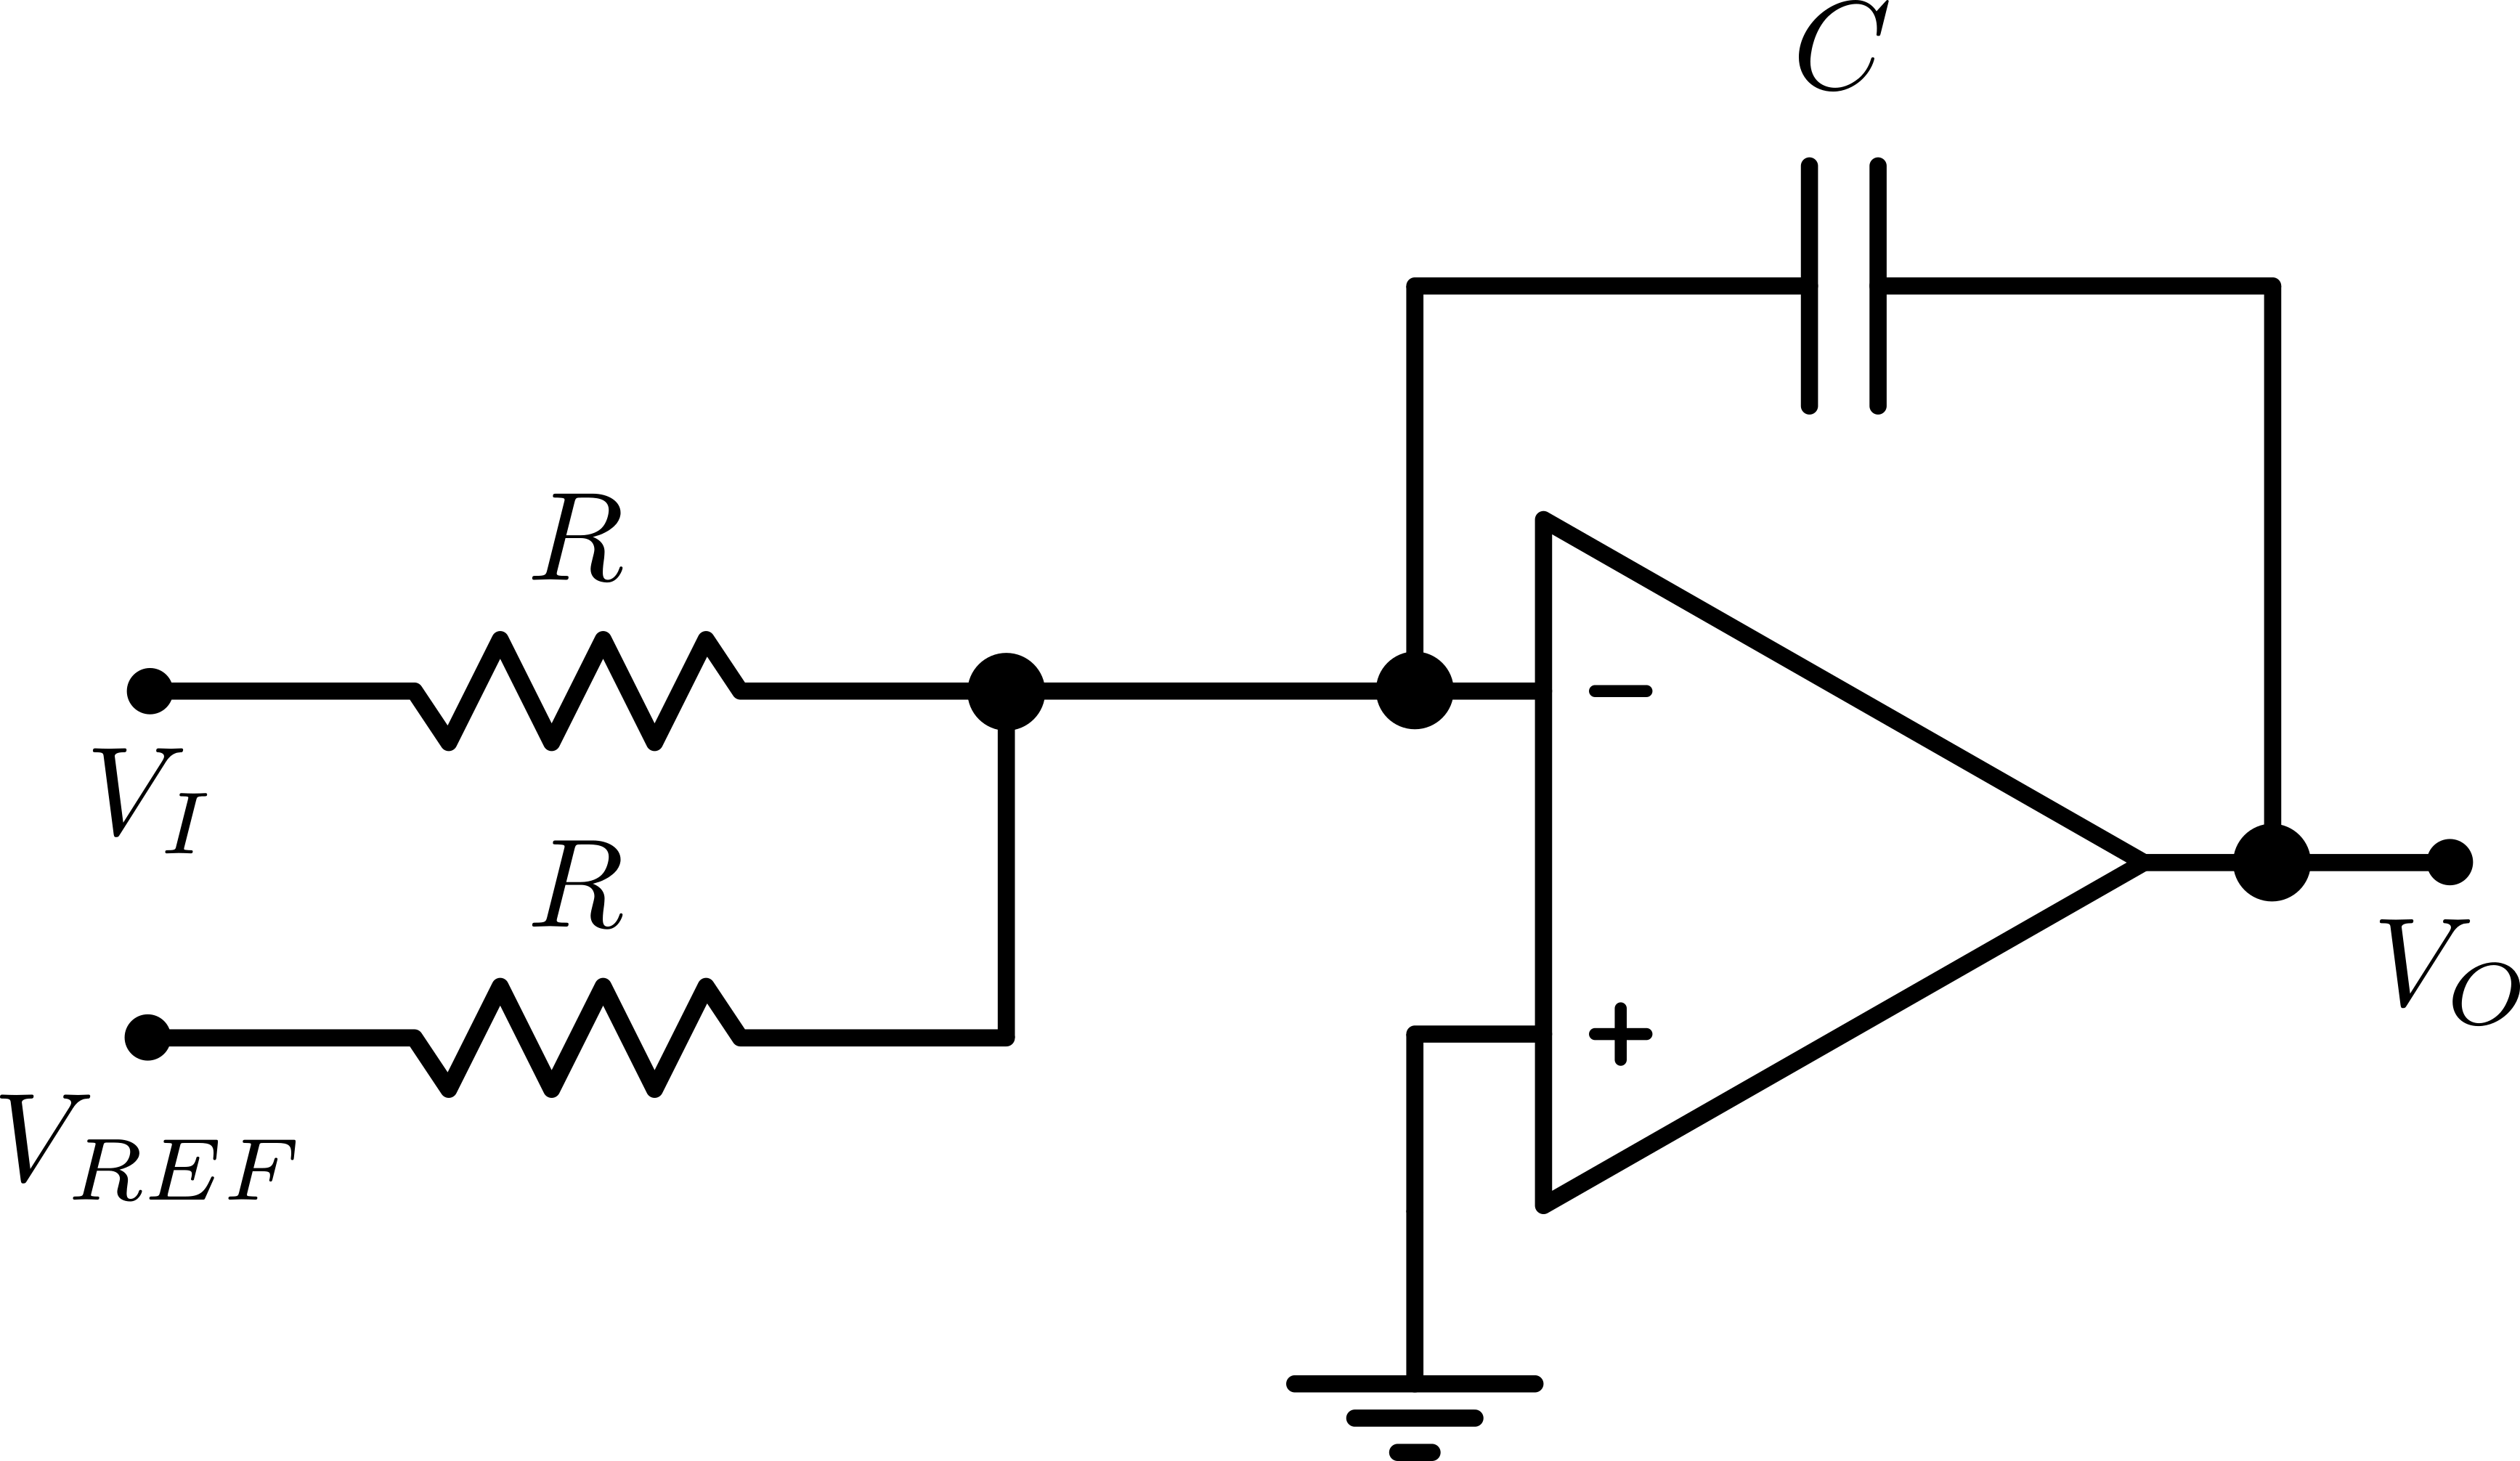
\includegraphics[scale=0.5]{images/ej5/IntegradorBasico.png}
\par\end{centering}
\caption{Circuito integrdor analógico}
\end{figure}


Aplicando la ganancia de tensión conocida para un circuito inversor con operacionales se tiene:

\[
V_O = (V_I+V_{REF}) \cdot \frac{-\frac{1}{sC}}{R} = (V_I + V_{REF}) \cdot -\frac{1}{sCR}
\]

En el caso propuesto, el circuito a implementar es diferencial, como se muestra a continuación.

\begin{figure}[!ht]
\begin{centering}
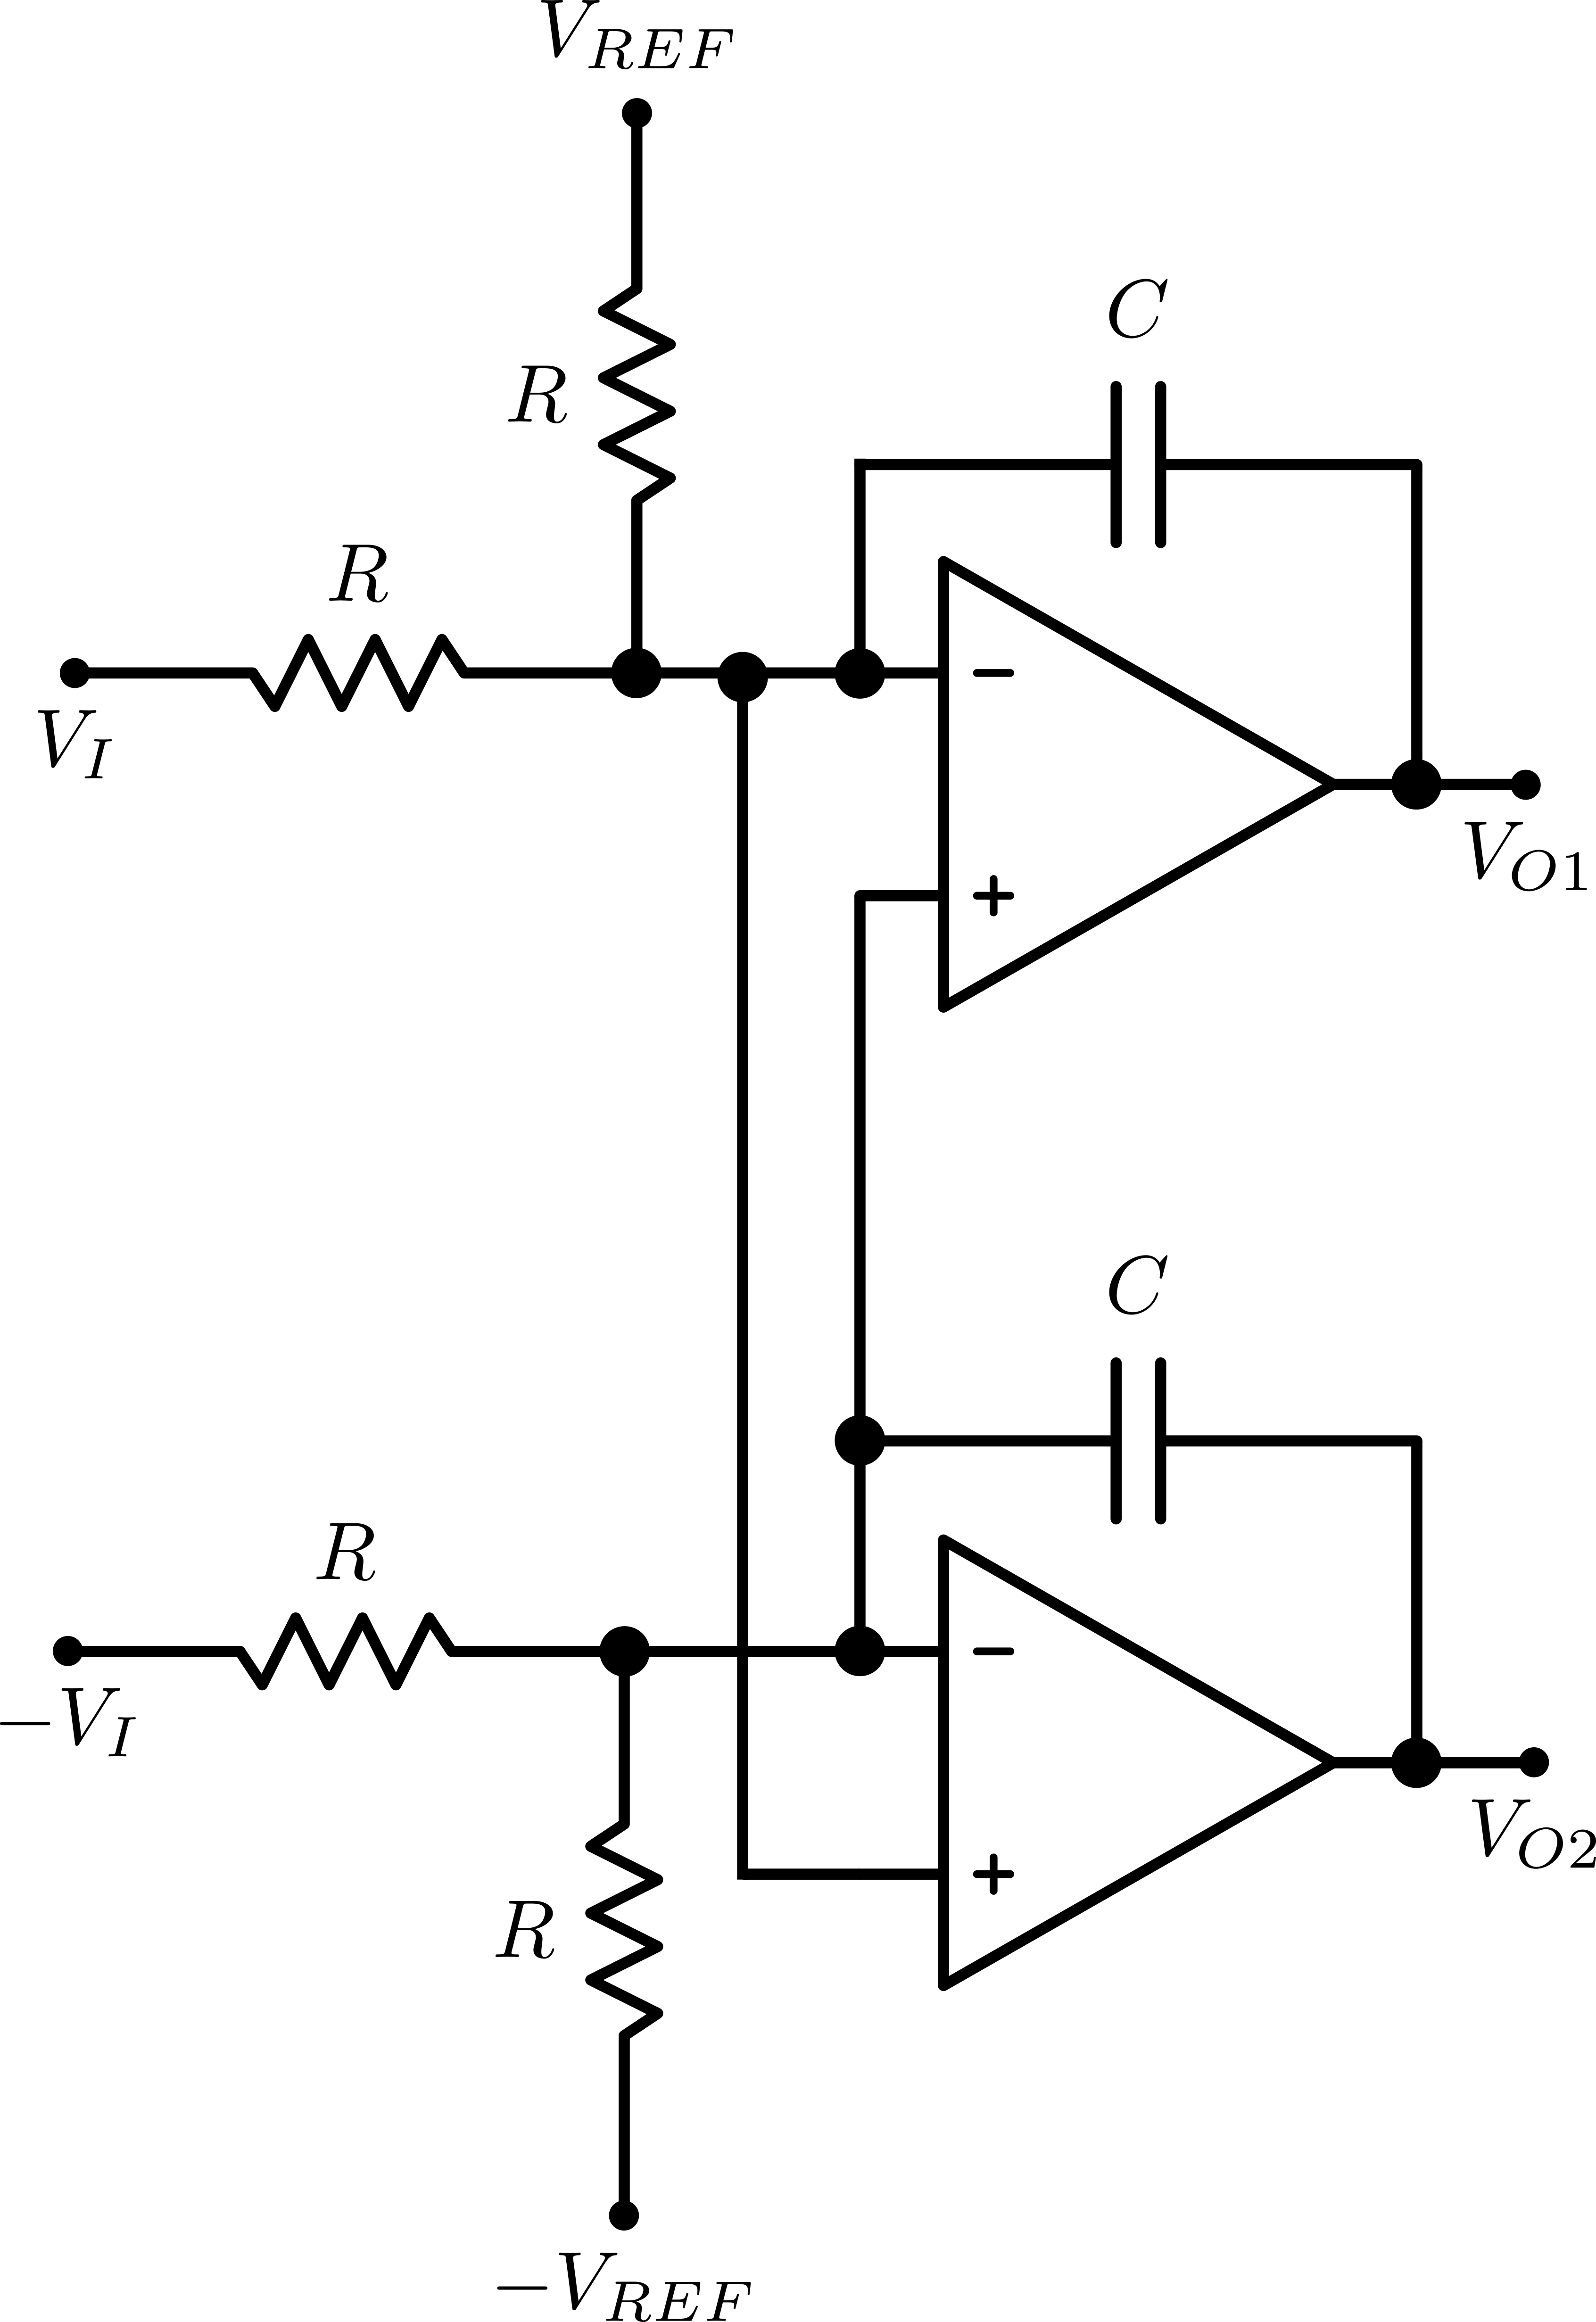
\includegraphics[scale=0.45]{images/ej5/IntegradorDif.png}
\par\end{centering}
\caption{Circuito integrdor diferencial}
\end{figure}

Como se mostró al inicio en el diagrama en bloques, se toma para una realimentación la salida $Q$ (pasada por el DAC) para un lazo y $\overline{Q}$ (también pasada por otro DAC idéntico) para el otro lazo (ya que al ser diferencial, ambos lazos deben ser complementarios). En este caso la salida a considerar $V_{O1} - V_{O2}$ no se observa en forma directa como en el circuito anterior. Pasivando por un lado las tensiones $V_{REF}$, se tiene planteando nodos:

\[
\left\lbrace
\begin{array}{l}
\dfrac{V_I-V_A}{R} + \dfrac{-V_A}{R} = (V_A-V_{O1}) \cdot sC \\
\\
\dfrac{-V_I-V_A}{R} + \dfrac{-V_A}{R} = (V_A-V_{O2}) \cdot sC
\end{array}
\right.
\] 

Restando ambas ecuaciones resulta:

\[
\frac{V_I}{sCR} = \frac{V_{O2}-V_{O1}}{2}
\]

Análogamente, pasivando las tensiones $V_{REF}$:

\[
\frac{V_{REF}}{sCR} = \frac{V_{O2}-V_{O1}}{2}
\]

Luego, por superposición, sumando ambos resultados se tiene finalmente:

\[
V_{O1} - V_{O2} = -\frac{1}{sCR} \cdot (V_I + V_{REF})
\]

Aplicando la transformación bilineal (que es la aproximación discreta de un integrador analógico):

\[
s \simeq \frac{2}{T} \cdot \frac{z-1}{z+1}
\]

Siendo T el período de muestreo. Resulta en la ecuación anterior:

\[
V_{O1}-V_{O2} = -\frac{V_I+V_{REF}}{CR} \cdot \frac{T}{2} \cdot \frac{z+1}{z-1}
\]
\newpage
Recordando ahora la equivalencia resistiva simulada del capacitor switcheado explicada al inicio (considerando ahora que son 4 switches y no 2, el período es la mitad):

\[
R = \frac{T}{2C_s}
\]

Si se reemplaza en la expresión anterior queda la aproximación al integrador analógico buscada:

\[
V_{O1}-V_{O2} = -\frac{V_I+V_{REF}}{C \cdot \dfrac{T}{2C_s}} \cdot \frac{T}{2} \cdot \frac{z+1}{z-1} = -(V_I + V_{REF}) \cdot \frac{C_s}{C} \cdot \frac{z+1}{z-1}
\]

El circuito que resulta de reemplazar la resistencia por el capacitor $C_s$ es:

\begin{figure}[!ht]
\begin{centering}
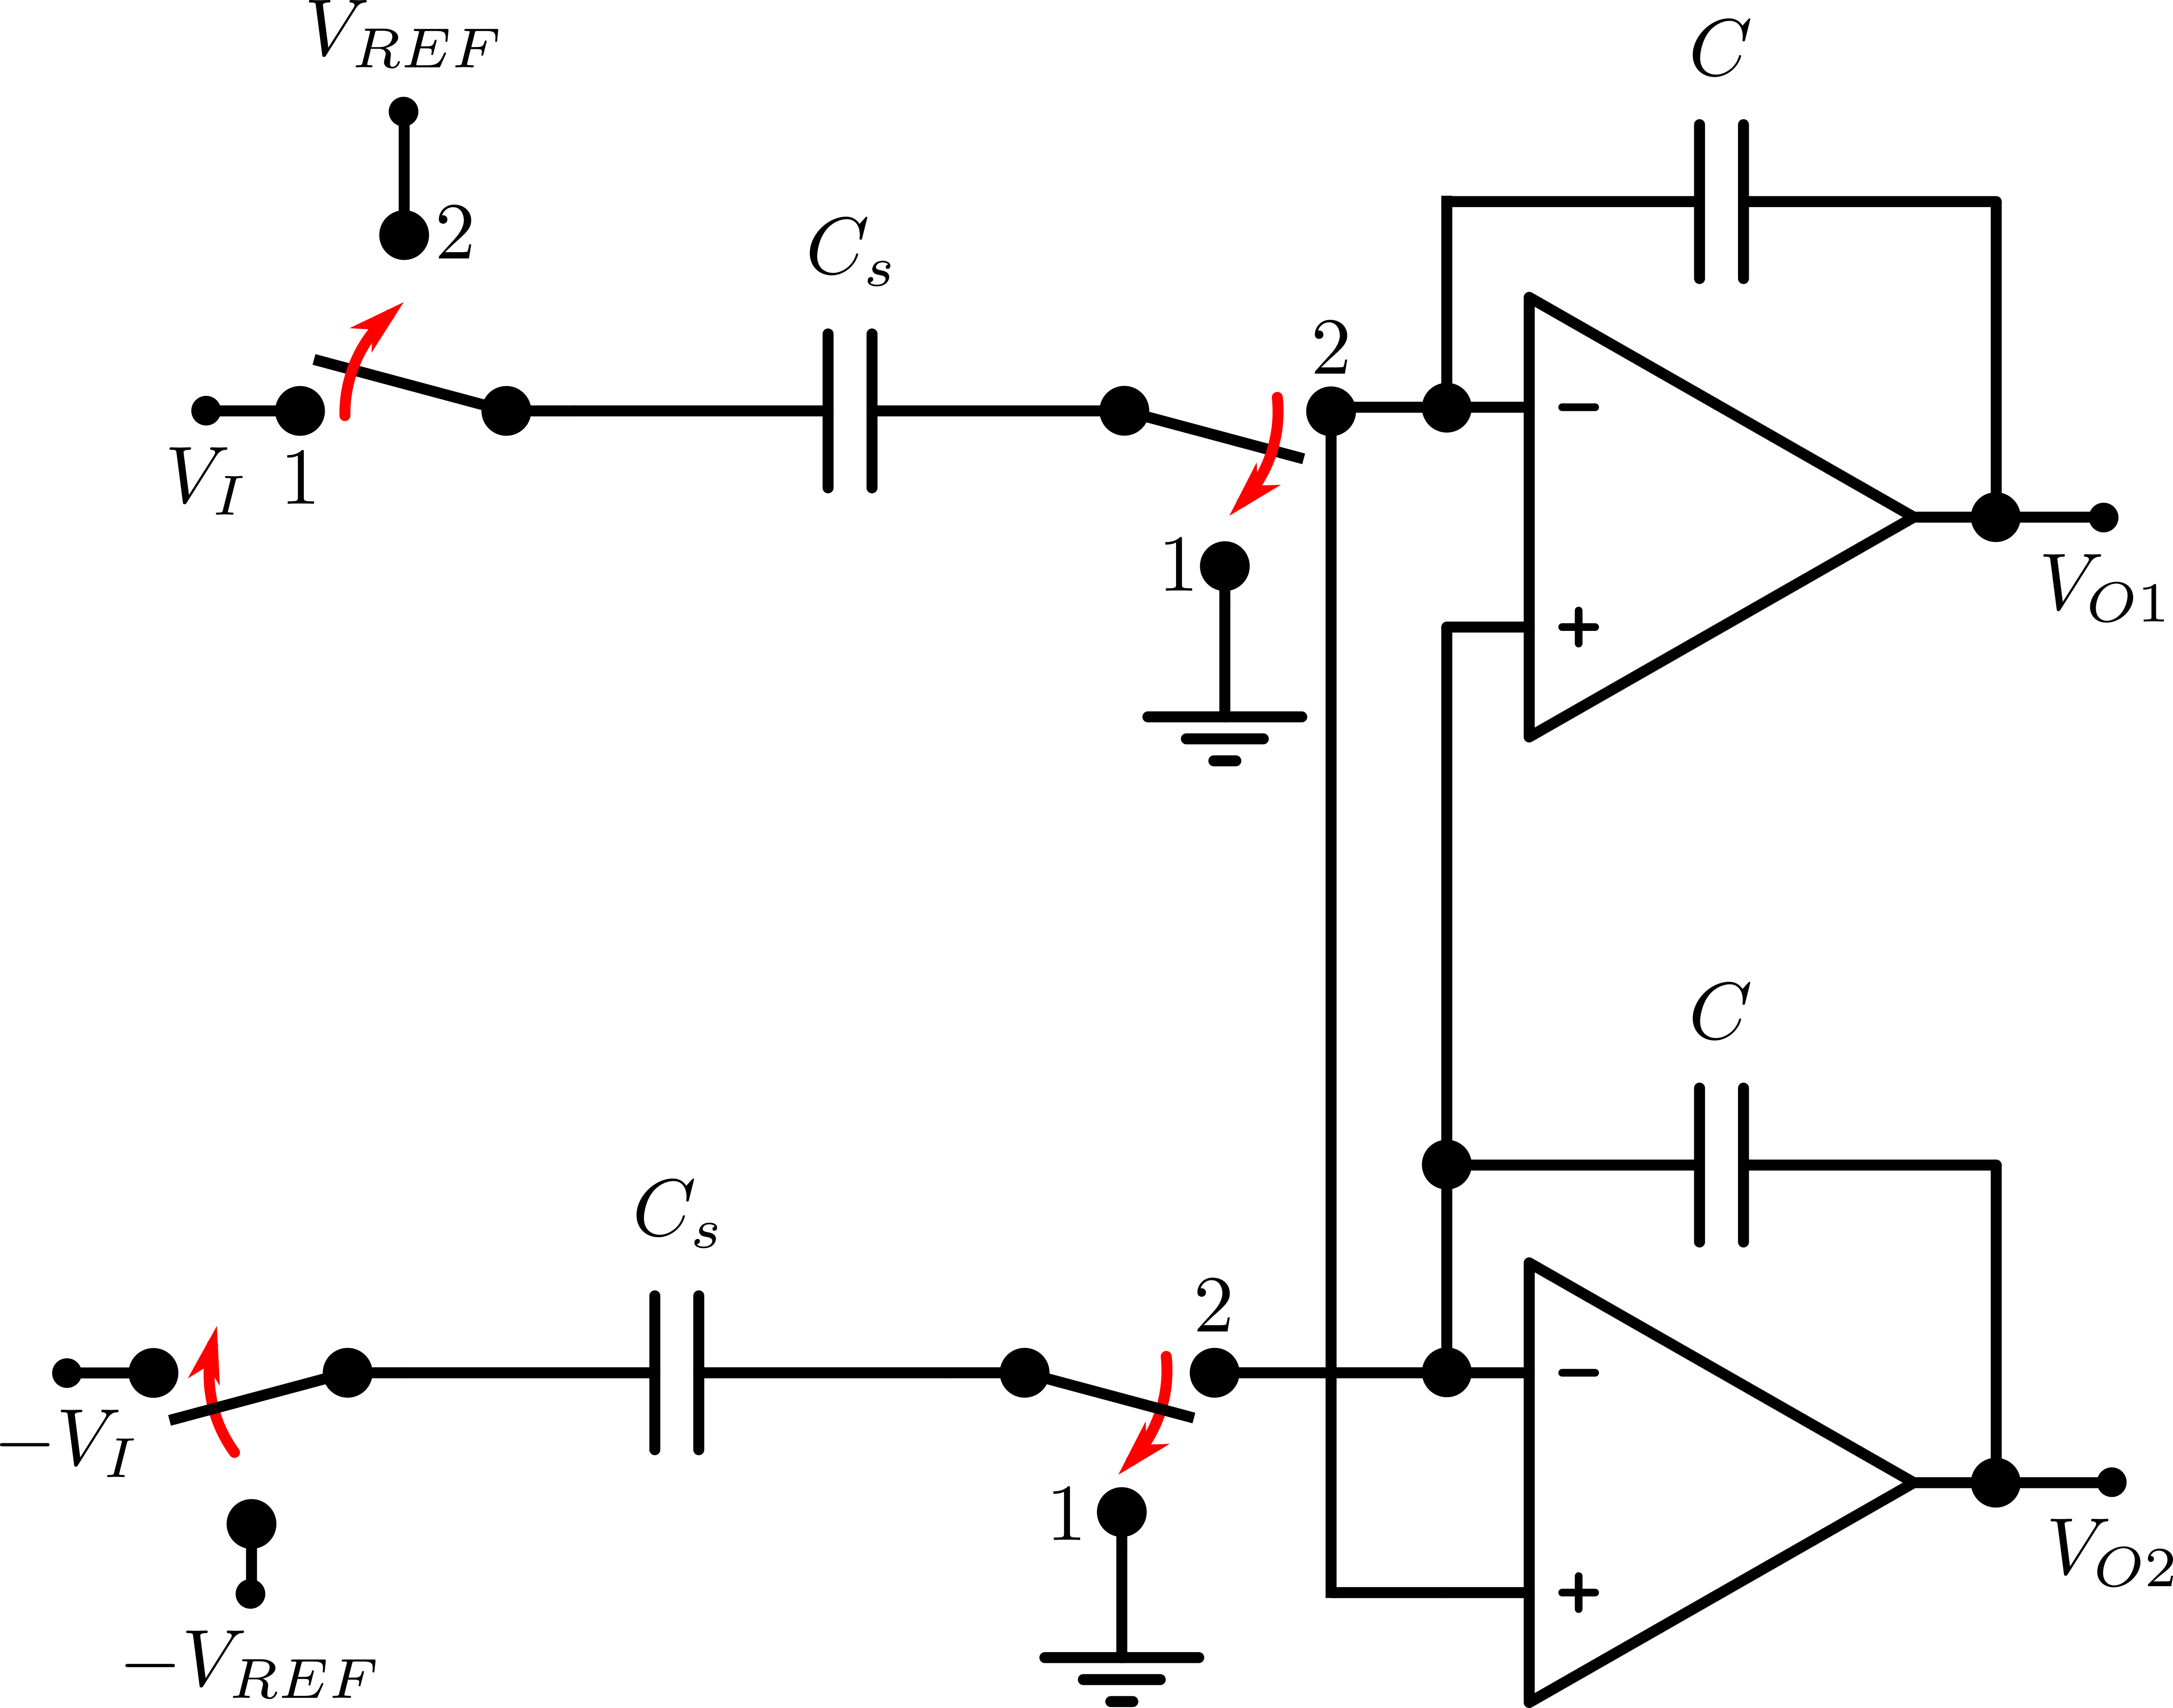
\includegraphics[scale=0.45]{images/ej5/IntegradorDifSC.png}
\par\end{centering}
\caption{Circuito integrador diferencial con SC}
\end{figure}

Las llaves $\phi$ se implementaron mediante multiplexores, utilizando la señal de clock como señal de control para la selección de las llaves. El multiplexor que se encontraba disponible es el CD4053.\par
En la bibliografía de apoyo utilizada (``Delta-Sigma Modulators: Modeling, Design and Applications'', George Bourdopoulos), en la sección 5.4 se describe una implementación de un modulador de primer orden para una frecuencia de sampleo similar a la mínima utilizada en este caso, sugiriendo un valor de $330pF$ para los capacitores del integrador SC. Por lo tanto, se adoptaron en primera instancia dichos valores ($C = C_s = 330pF$).

\subsubsection{Cuantizador de 1 bit}

Se toma la salida del integrador diferencial, y mediante un comparador a lazo abierto se implementa el cuantizador de 1 bit. El circuito implementado es utilizando el comparador LM311, y luego, dicha salida se conecta a un flip-flop D, el cual actúa como latch. El flip-flop D utilizado es el integrado CD4013, alimentado entre +5V y 0V. La alimentación adicional se obtuvo a partir de la entrada de +15V del circuito pasándola un regulador LM7805.

\begin{figure}[!ht]
\begin{centering}
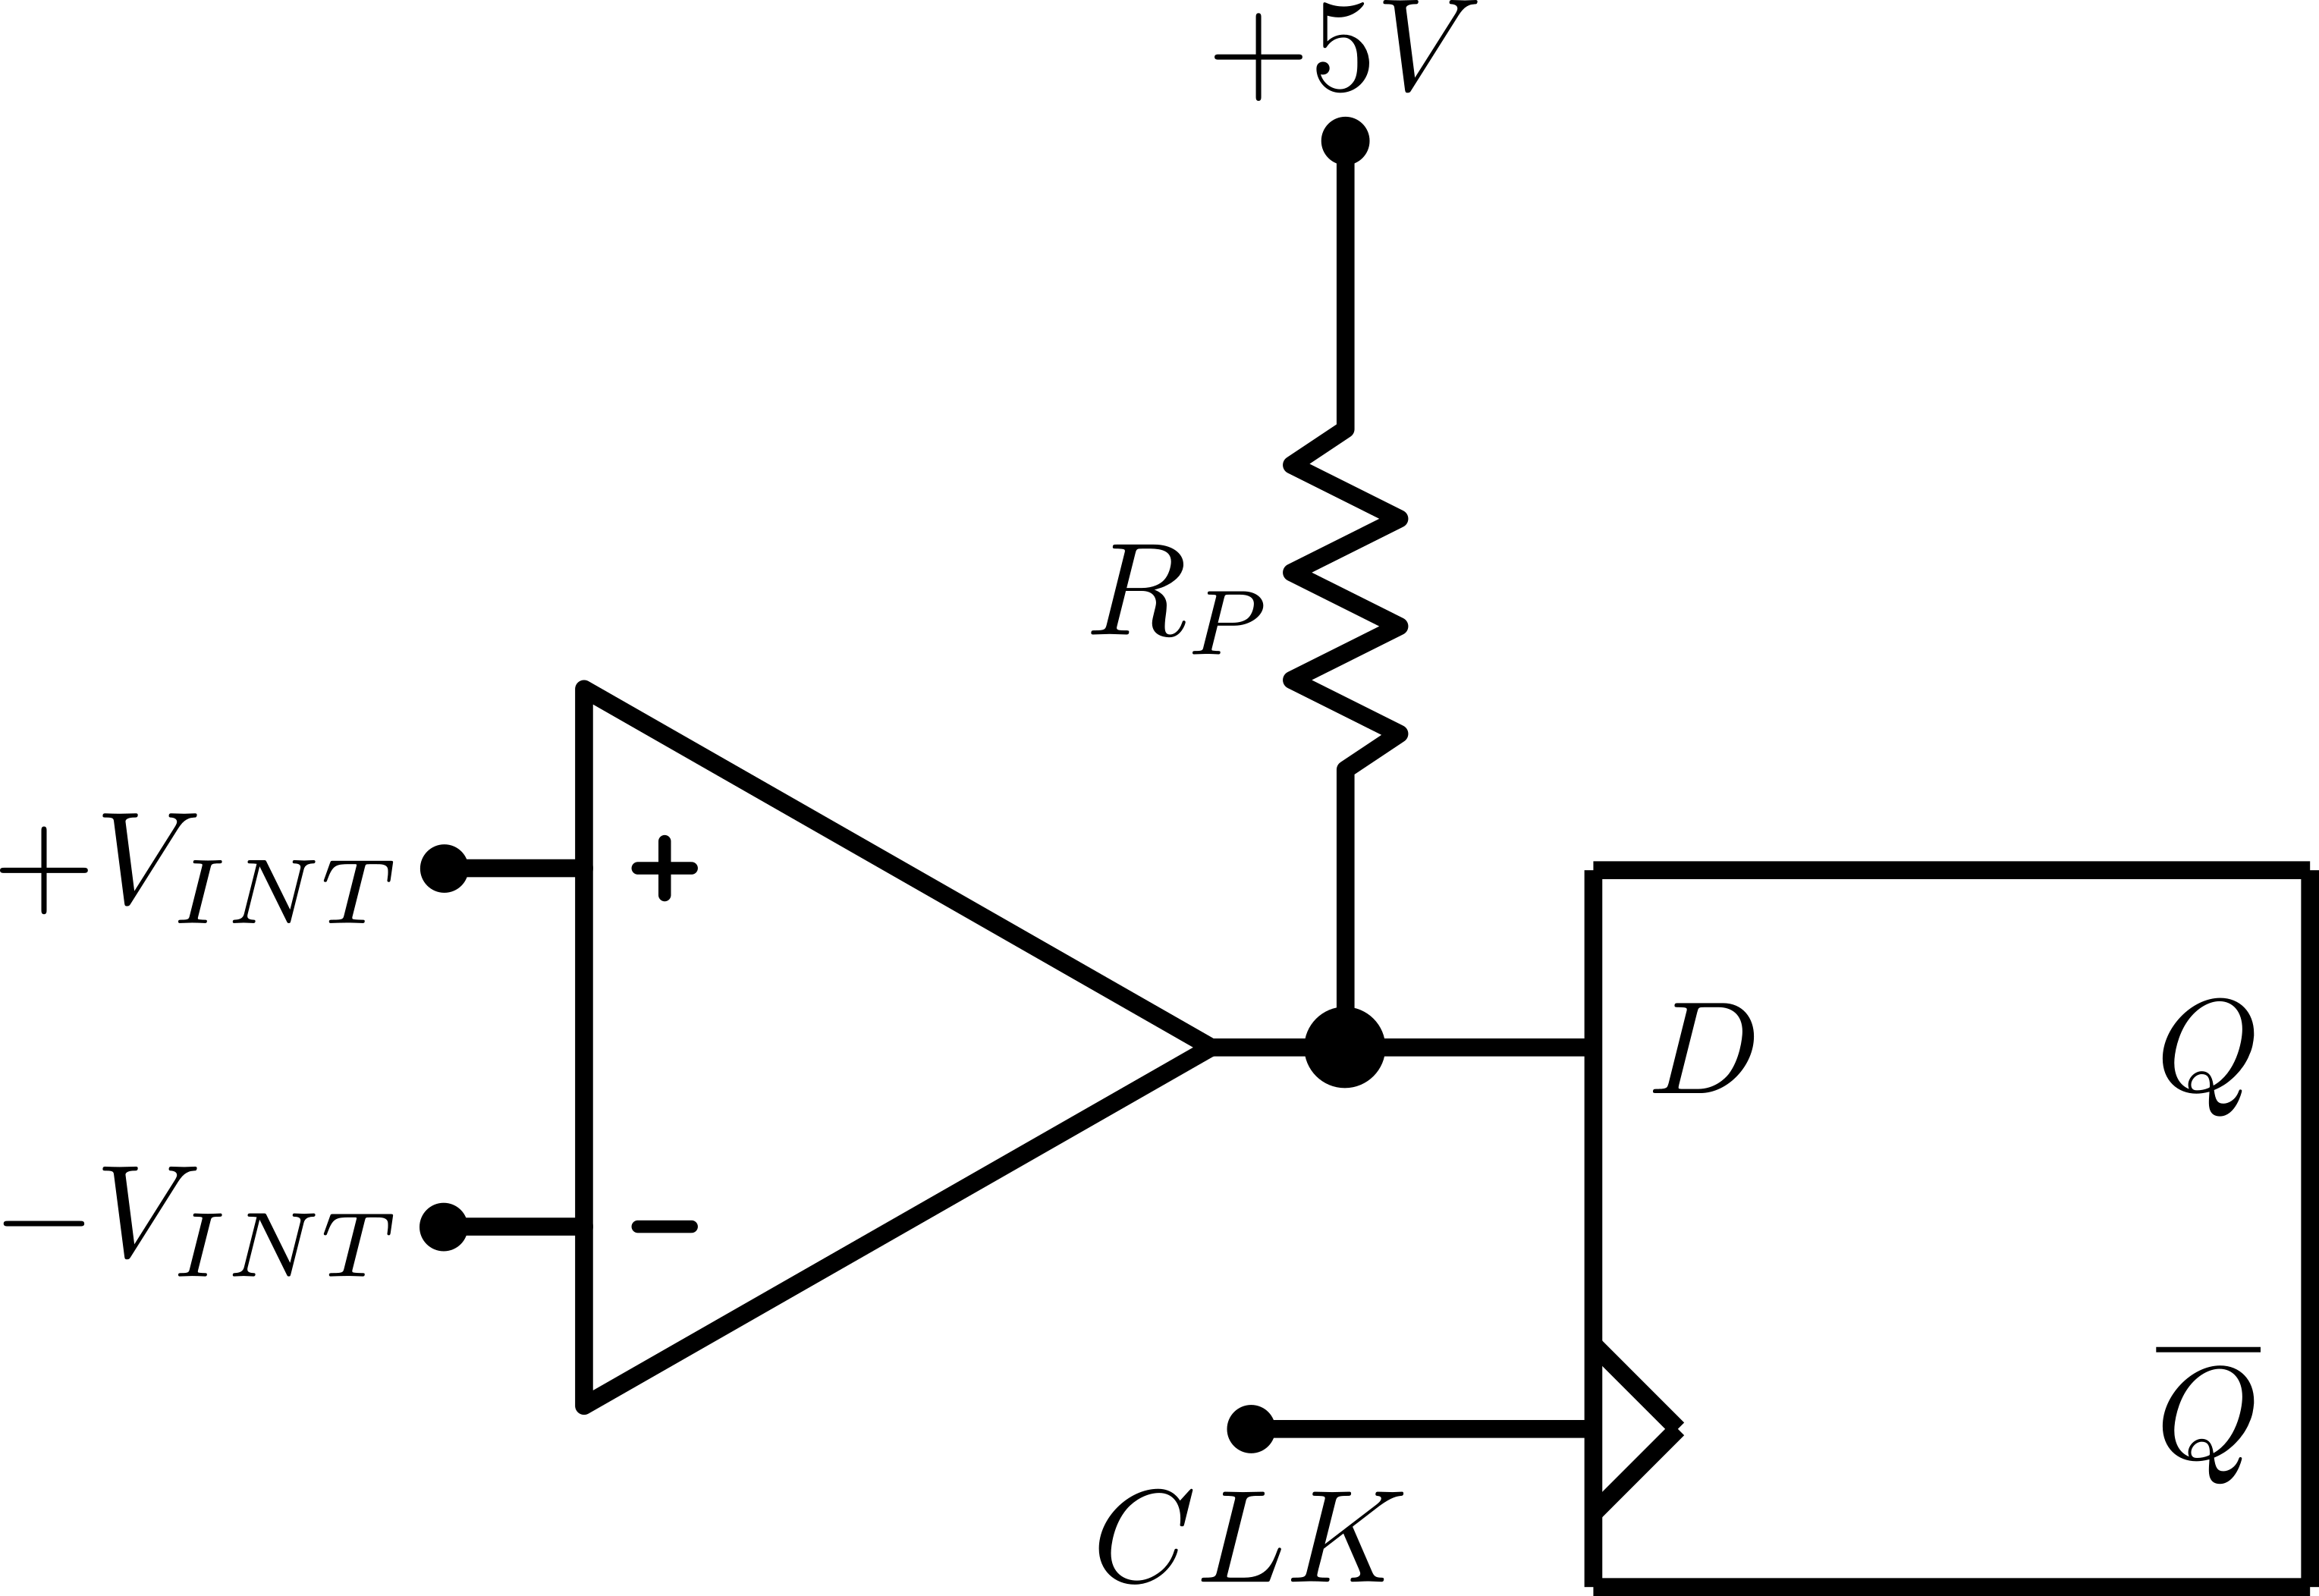
\includegraphics[scale=0.5]{images/ej5/Comp.png}
\par\end{centering}
\caption{Cuantizador 1 bit}
\end{figure}

Como se mostrará en las mediciones obtenidas, la salida que se obtiene en este punto del circuito es una señal cuadrada de ancho de pulso modulado (PWM). En los tramos donde la pendiente de la señal es pequeña, las variaciones en la salida del integrador serán menores, por lo que en consecuencia el ancho de los pulsos resultantes es mayor. En los tramos donde la pendiente de la señal es mayor, las variaciones a la salida del integrador son más frecuentes, por lo que el ancho de los pulsos es menor.

\subsubsection{DAC para realimentación}

Las salidas binarias del flip-flop D corresponden a 0V (0 lógico), y +5V (1 lógico). Esta salida (tanto $Q$ y $\overline{Q}$) son convertidas mediante un DAC a -5V (0 lógico) y +5V (1 lógico), siguiendo el esquema propuesto por la bibliografía. Cada DAC es implementado mediante un multiplexor, utilizando las salidas del flip-flop como señales de control.

\begin{figure}[!ht]
\begin{centering}
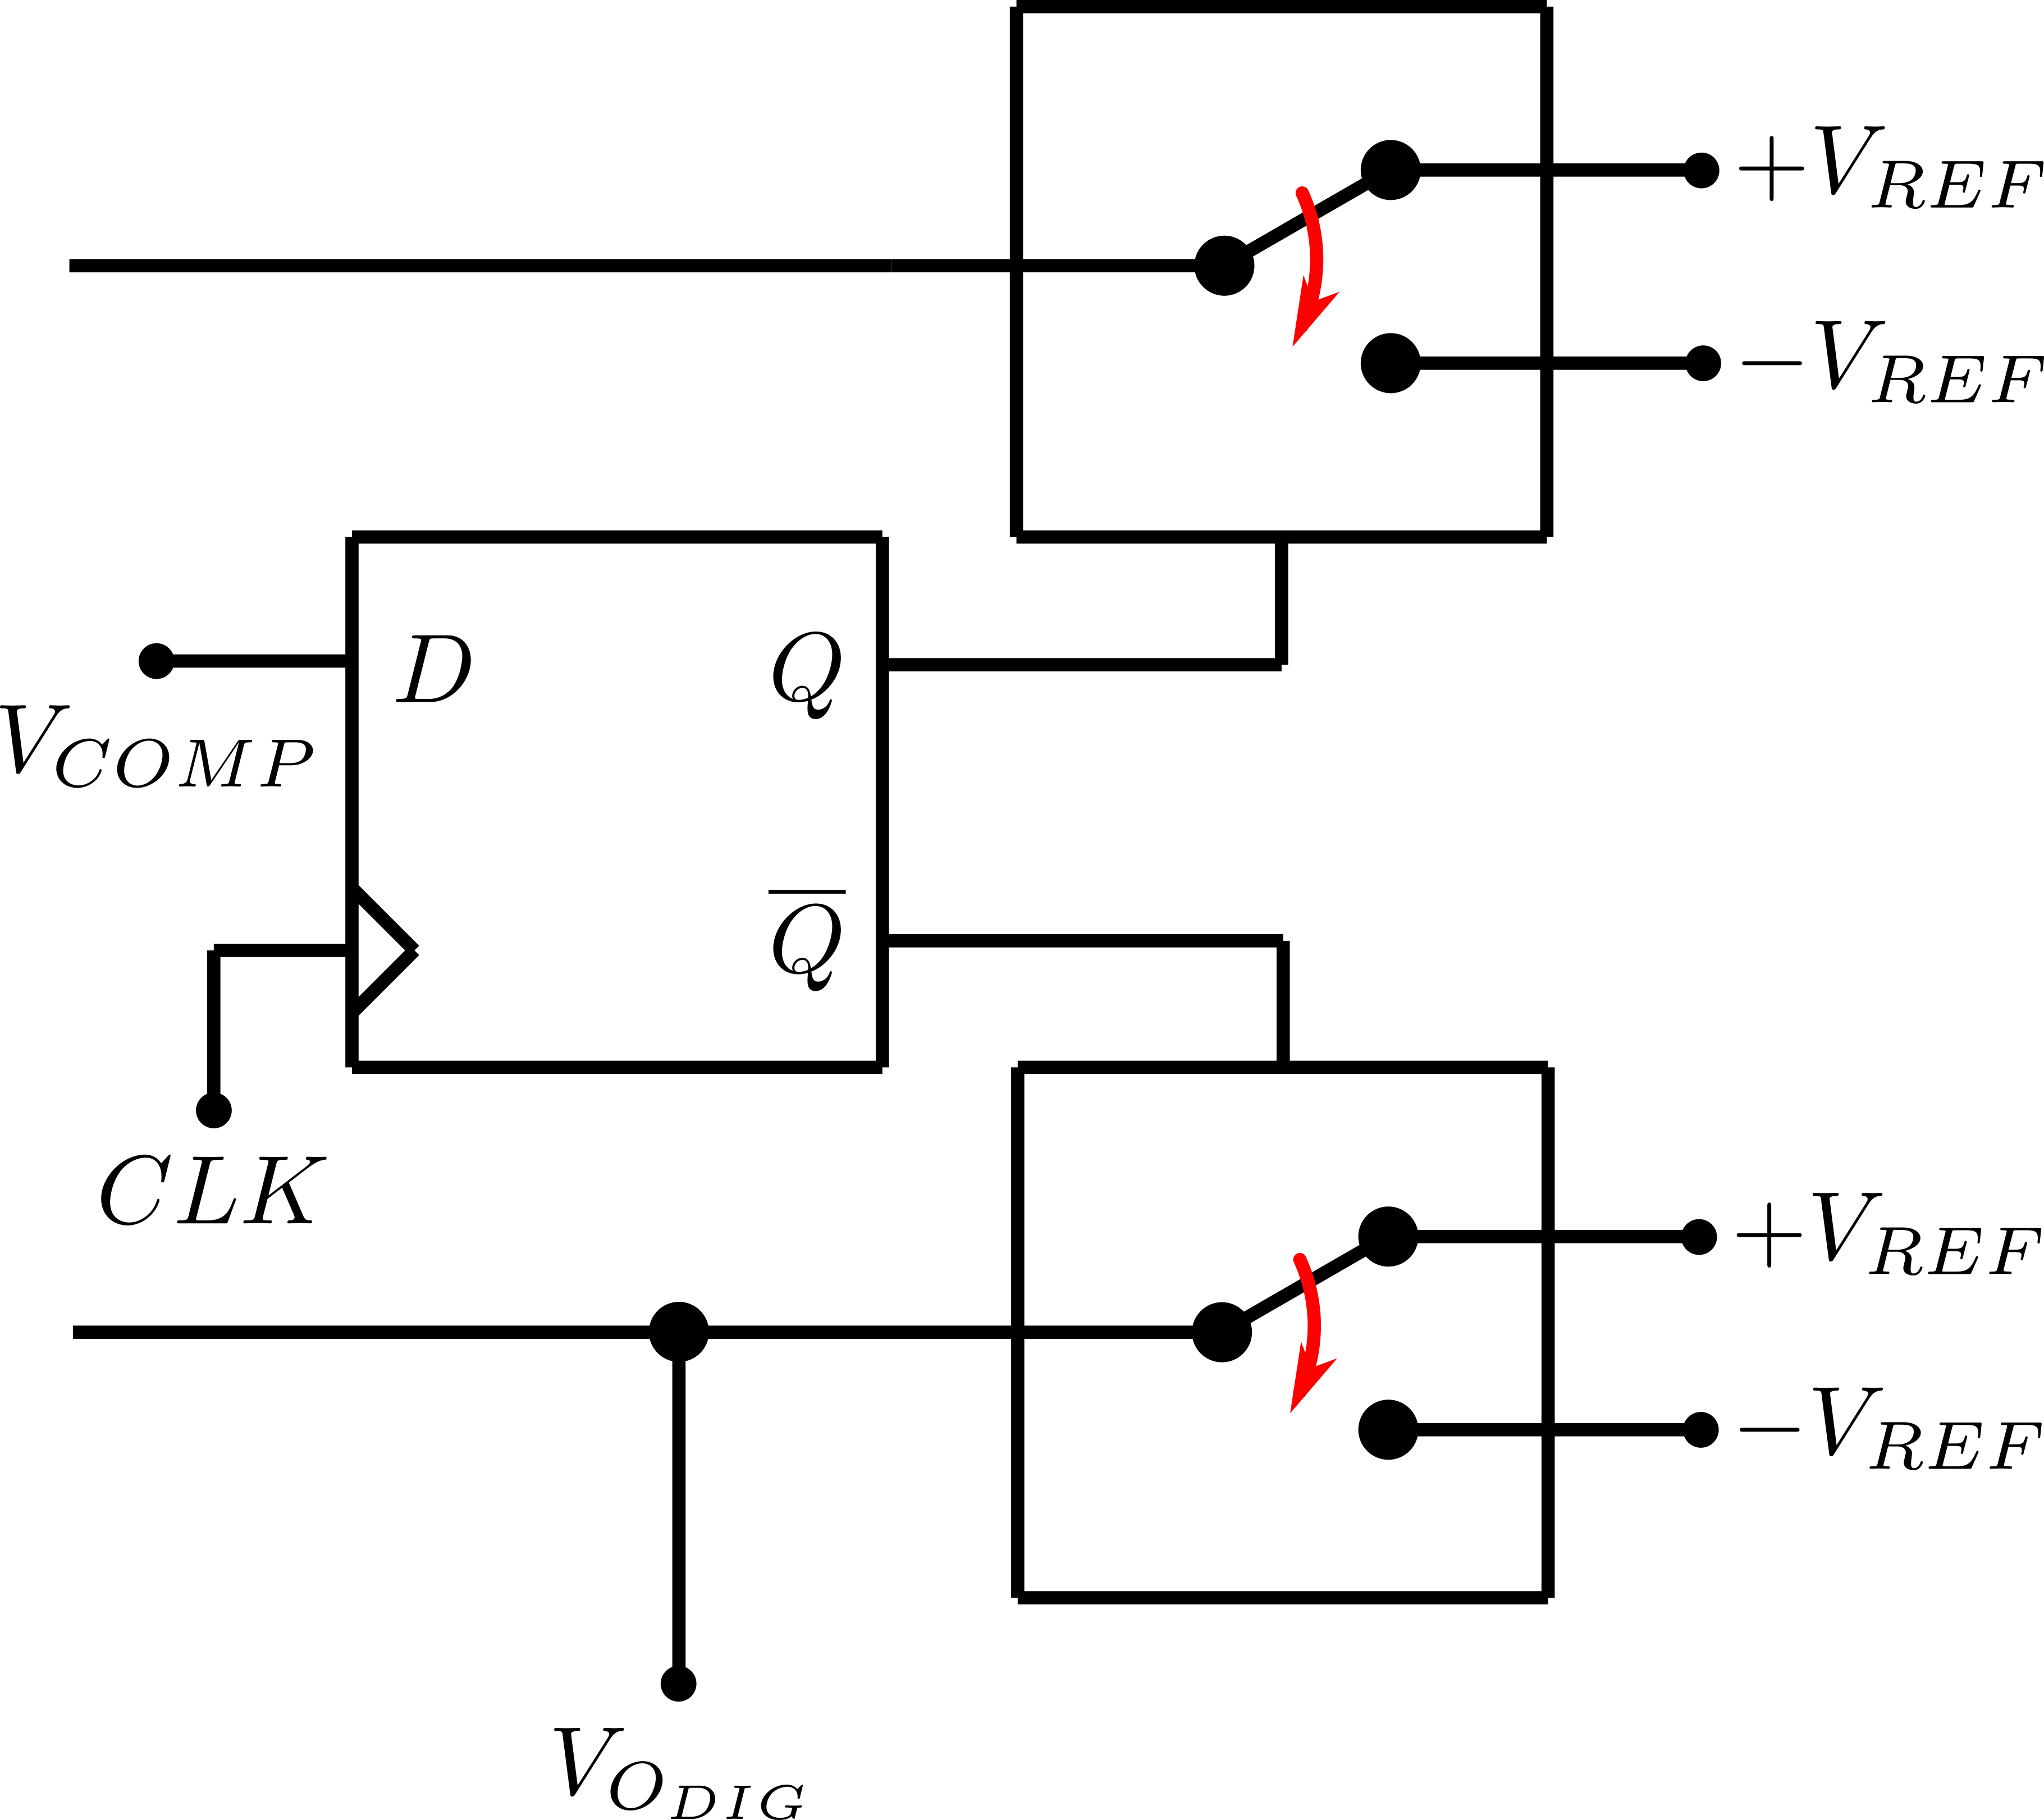
\includegraphics[scale=0.5]{images/ej5/DAC.png}
\par\end{centering}
\caption{DAC de [0V +5V] a [-5V +5V]}
\end{figure}

Se toma la salida de uno de los DAC como señal digital, para luego procesarla por el filtro recuperador (idéntico al antialiasing), para volver a obtener la señal original al quedarnos sólo con el espectro en banda base.
\newpage
\subsection{Mediciones - Resultados obtenidos}

Al realizar las mediciones con señales senoidales de prueba, se observó que la señal recuperada se encontraba invertida respecto a la señal de entrada. Esto se debe a un pequeño error en el esquemático del PCB, donde se conectaron en forma inversa las salidas del diferenciador a las entradas del integrador diferencial. Para solventar esto, se utilizó la función Invert del osciloscopio sobre el canal que mide la salida.

\subsubsection{Senoidal}

Para este caso, se logró utilizar una senoidal de entrada de 10Vp, y como frecuencia máxima se tomó una un poco menor (5KHz) a la de corte del filtro antialias (que se encuentra en 6KHz, para evitar los 3dB de máximo error de la respuesta en frecuencia real). En este caso, también se buscó probar el muestreo a máxima frecuencia, es decir a MHz. Los resultados en los distintos puntos del circuito se muestran a continuación.

\begin{figure}[!ht]
\begin{centering}
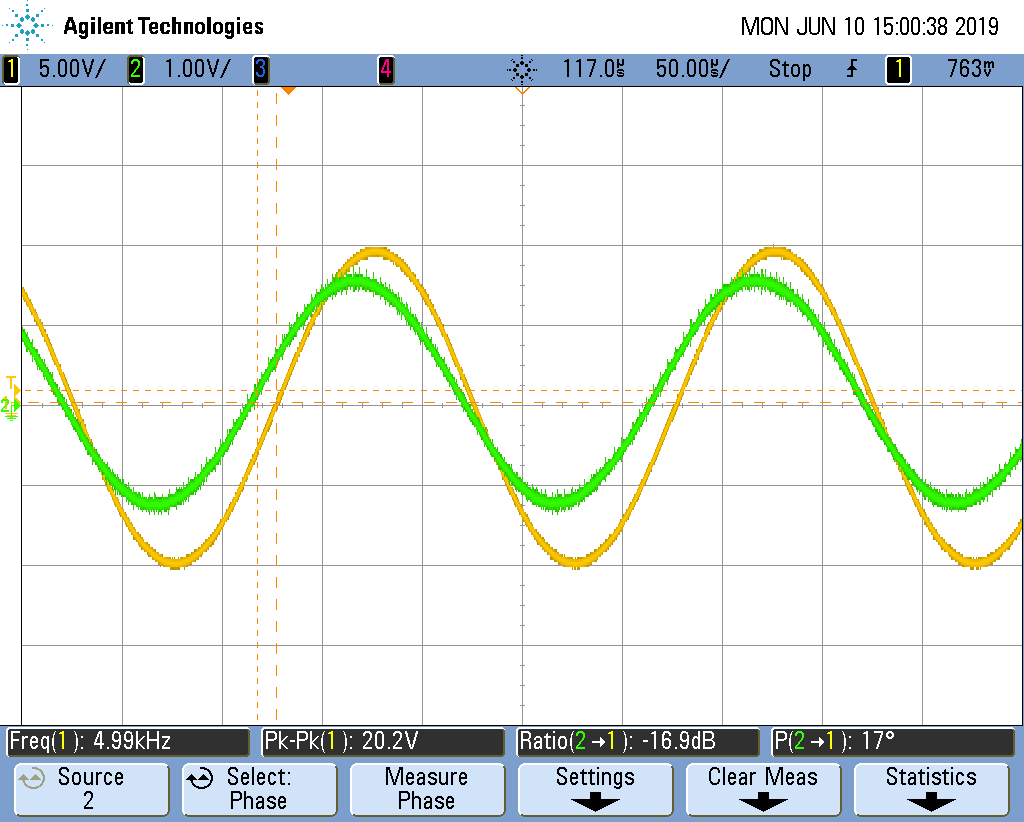
\includegraphics[scale=0.25]{../EJ4/Mediciones/Seno/s1_1.png}
\par\end{centering}
\caption{Señal de entrada y recuperada - Atenuación y desfasaje (CH1: Entrada, CH2: Salida)}
\end{figure}

Se observa que la señal recuperada sigue la forma senoidal de la entrada, aunque atenuada. Dado que el espectro de la senoidal ideal son dos deltas a la frecuencia de oscilación, no se pierden armónicos en el filtro antialias. Por lo tanto, al filtrar las repeticiones del espectro a la salida y quedarse solamente con la banda base, se esperaba obtener una buena representación, como efectivamente se observó. En este caso, al estar la frecuencia de sampleo en 1MHz, la atenuación de la primer repetición del espectro ya resulta mayor a 80dB.

\begin{figure}[!ht]
\begin{centering}
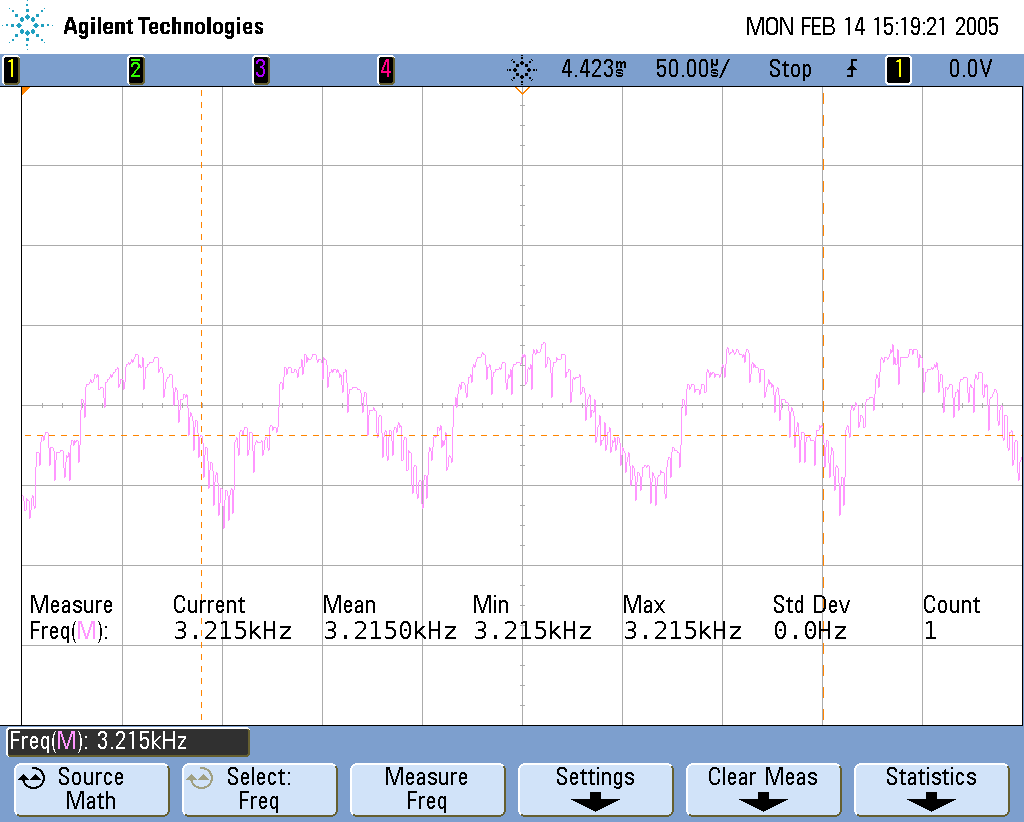
\includegraphics[scale=0.25]{../EJ4/Mediciones/Seno/dif_seno.png}
\par\end{centering}
\caption{Señal de entrada y salida diferencial - (CH1: Entrada, CH2: Salida diferencial)}
\end{figure}

Se tomaron las dos salidas del integrador diferencial, y mediante la función Math del osciloscopio se hizo la diferencia. El resultado que se observa en la figura tiene una frecuencia fundamental similar a la senoidal original, y se corresponde con la integral de la senoidal (que es de la misma forma) sumada a la respuesta a la señal cuadrada de la realimentación del DAC.

\begin{figure}[!ht]
\begin{centering}
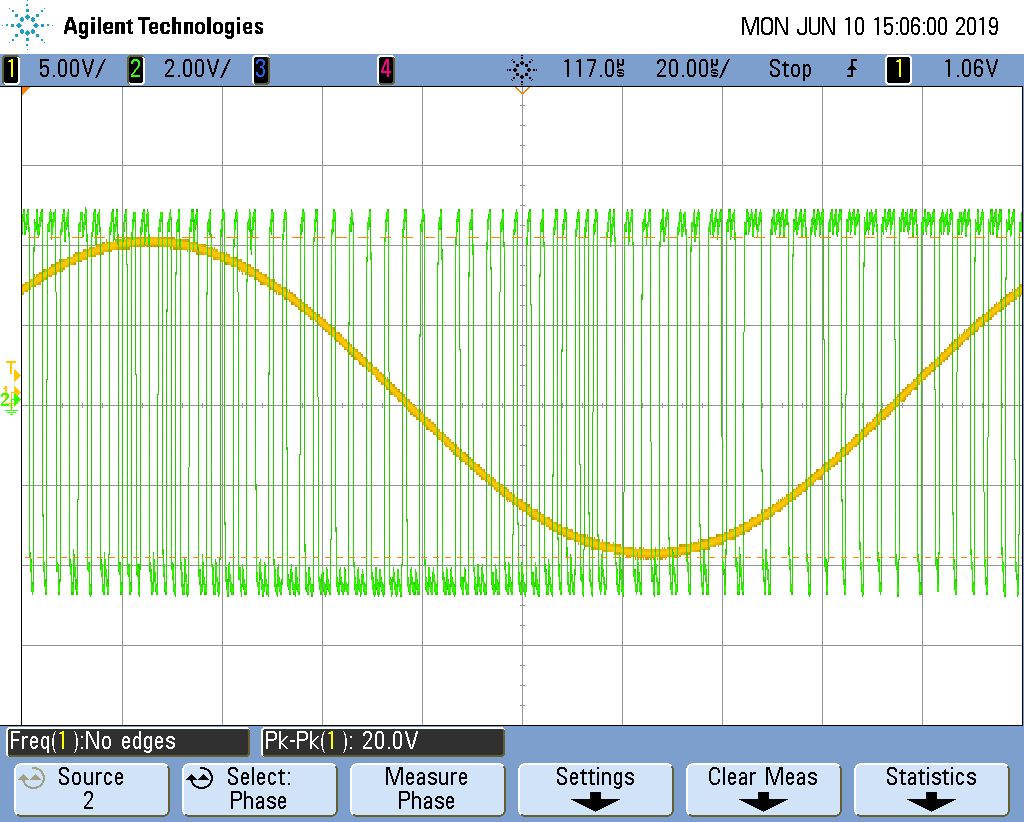
\includegraphics[scale=0.25]{../EJ4/Mediciones/Seno/s1_3.png}
\par\end{centering}
\caption{Señal de entrada y salida digital - (CH1: Entrada, CH2: Salida digital)}
\end{figure}

La señal obtenida del comparador resulta una cuadrada de ancho de pulsos variables, como se mencionó en la implementación. Los pulsos resultan anchos en las cercanías de los picos de la senoidal (dado que allí la variación es más leve), mientras que en torno a donde la señal cruza por cero la variación es máxima, y el ancho de los pulsos resulta menor.

\begin{figure}[!ht]
\begin{centering}
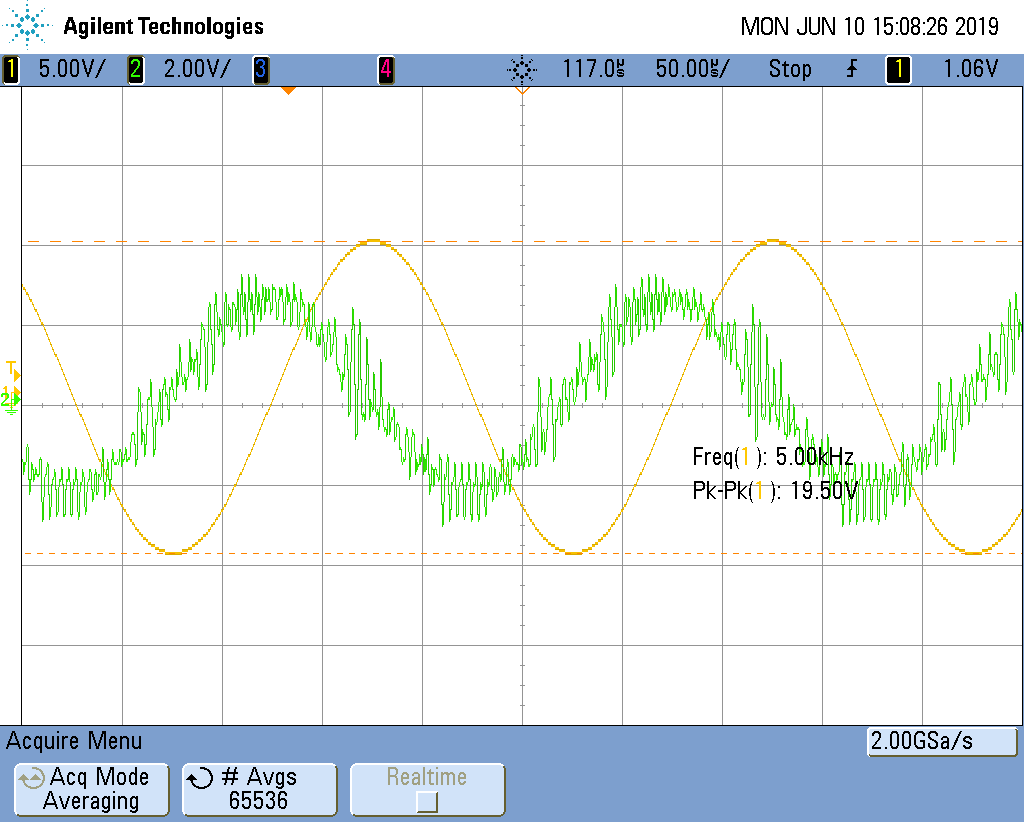
\includegraphics[scale=0.25]{../EJ4/Mediciones/Seno/s1_4.png}
\par\end{centering}
\caption{Señal de entrada y salida digital - (CH1: Entrada, CH2: Salida digital con average máximo)}
\end{figure}

Al utilizar el promediador del osciloscopio, en forma aproximada se filtra la señal digital, dejando solamente componentes en bajas frecuencias, lo que resulta en una señal que se asemeja a la de la entrada. Sin embargo, en comparación a la señal recuperada con el filtro de la placa, la promediada en el osciloscopio pierde más amplitud. Esto se debe a que lo que se realiza en este caso no es filtrado del espectro en sí, sino una promediación de una cierta cantidad de muestras tomadas de la señal, lo que inevitablemente lleva a perder un poco de información.

\newpage

\begin{figure}[!ht]
\begin{centering}
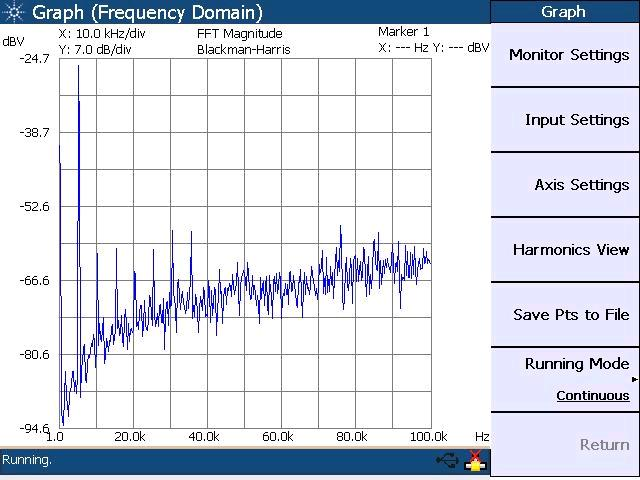
\includegraphics[scale=0.55]{../EJ4/Mediciones/Seno/s1_ns.jpeg}
\par\end{centering}
\caption{Visualización de efecto de noise shaping en la señal digital}
\end{figure}

Tomando la señal digital, en el espectro obtenido del analizador de espectros se observa que en bajas frecuencia se tiene la mayor atenuación, y a medida que se aumenta la frecuencia la atenuación es cada vez menor, visualizando el efecto de noise shaping. Por otra parte, se puede observar también en forma notoria el espectro de la senoidal en banda base, correspondiente a la delta de dirac en aproximadamente 5KHz.

\subsubsection{1/2 Gauss}
En este caso, considerando que se pedía una frecuencia mínima de 2.5KHz, se utilizó una cercana (3KHz - 5Vp) de forma tal de poder conservar la mayor cantidad de armónicos posibles al pasar por el filtro antialias (dado que la frecuencia de corte es fija). Sin embargo, dado el gran ancho de banda de esta señal (como ya se explicó), se pierde una parte considerable de la potencia de la misma, por lo que el salto tipo escalón resultará visiblemente atenuado.

\begin{figure}[!ht]
\begin{centering}
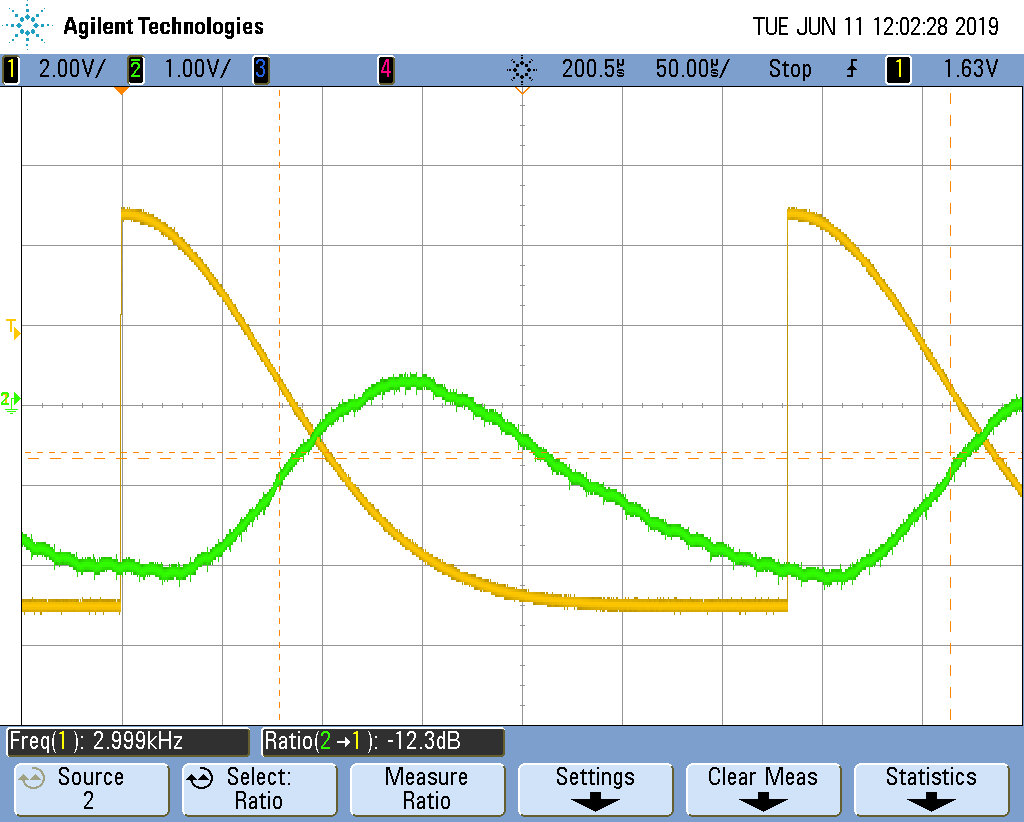
\includegraphics[scale=0.25]{../EJ4/Mediciones/0.5Gauss/s2_1a.png}
\par\end{centering}
\caption{Señal de entrada y recuperada - Atenuación (CH1: Entrada, CH2: Salida)}
\end{figure}

Para esta señal y la siguiente, se utilizó un factor de oversampleo L = 64, el mínimo comunmente utilizado. Considerando la frecuencia de la señal a 3KHz, la frecuencia para cumplir con Nyquist es de 6KHz. Multiplicando por el factor L, resulta en una frecuencia de oversampling de aproximadamente 400KHz. Por lo tanto, se configuró el clock a dicha frecuencia.\par
Como era de esperar, la sección del salto resultó bastante atenuada. Midiendo el defasaje temporal con cursores, las señales resultaron desfasadas en aproximadamente $30^{\circ}$.
\newpage
\begin{figure}[!ht]
\begin{centering}
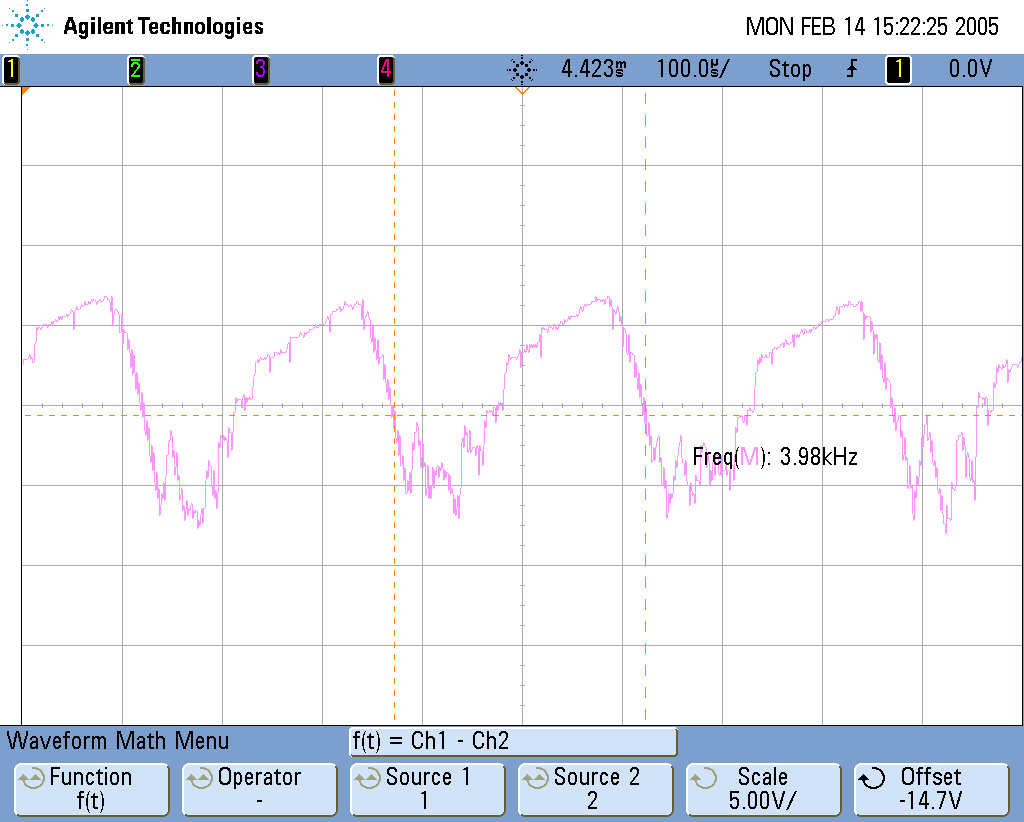
\includegraphics[scale=0.25]{../EJ4/Mediciones/0.5Gauss/dif_gaus.png}
\par\end{centering}
\caption{Señal de entrada y salida diferencial - (CH1: Entrada, CH2: Salida diferencial)}
\end{figure}

En este caso se procedio de igual manera que para la señal senoidal, tomando la salida diferencial del integrador, y haciendo la resta mediante la función Math. La señal obtenida tiene características similares a lo mencionado para la senoidal. También mantiene una forma similar a la 1/2 de gauss, pero como se encuentra invertida por lo explicado al principio (y en Math no se puede usar la función de inversión) no se puede comparar a simple vista.

\begin{figure}[!ht]
\begin{centering}
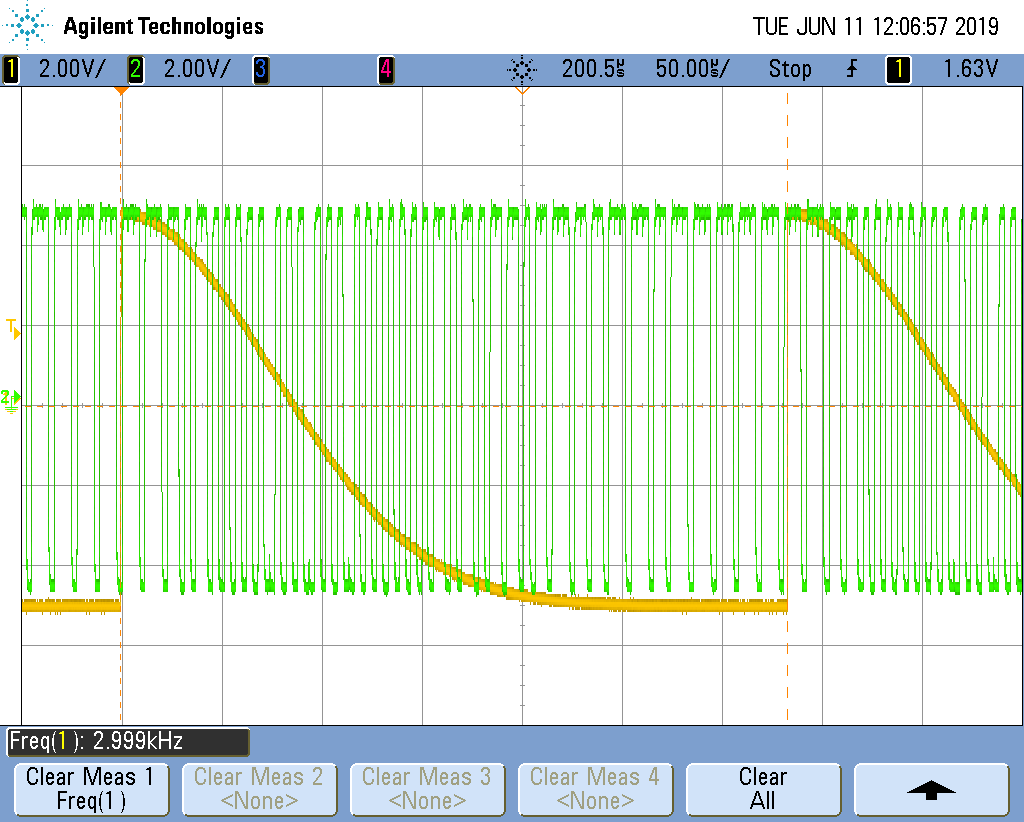
\includegraphics[scale=0.25]{../EJ4/Mediciones/0.5Gauss/s2_3.png}
\par\end{centering}
\caption{Señal de entrada y salida digital - (CH1: Entrada, CH2: Salida digital)}
\end{figure}

En este caso, al usar una frecuencia de sampleo menor, logra apreciarse lo comentado previamente sobre las variaciones de ancho de pulso. Se puede observar claramente en este caso, donde mayor pendiente posee la gaussiana más oscilaciones resultan (debido a menor ancho de pulso), y éstos se van agrandando a medida que pierde pendiente en forma monótona.
\newpage
\begin{figure}[!ht]
\begin{centering}
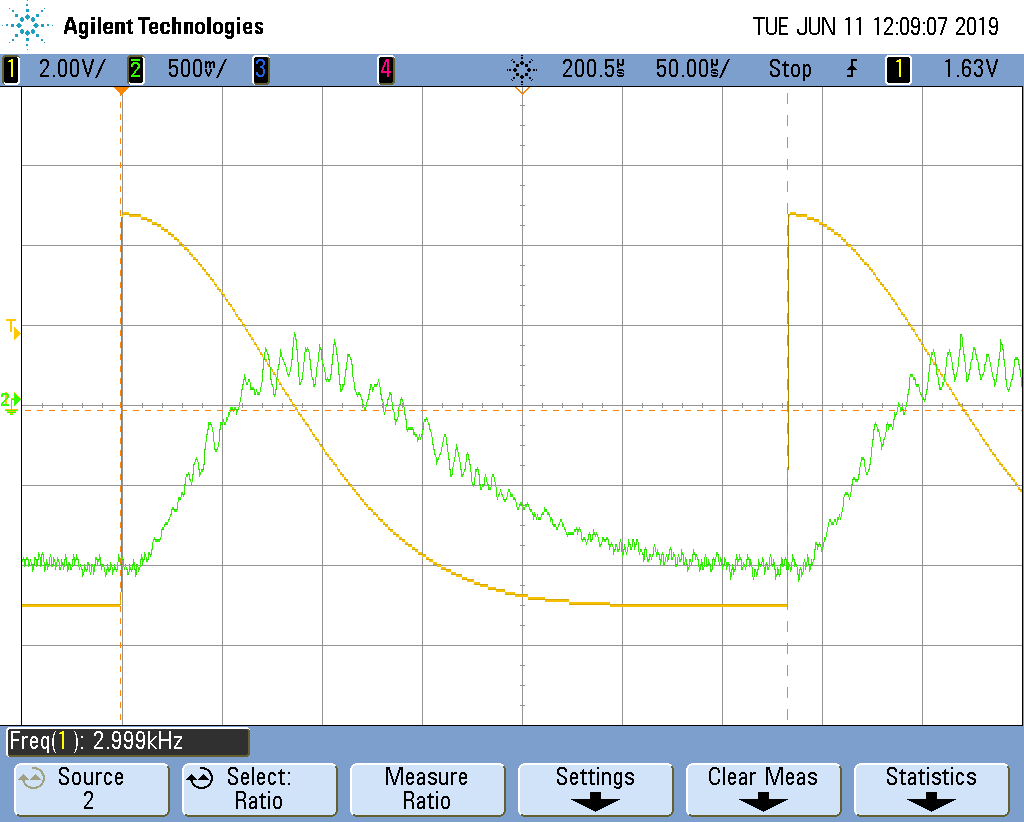
\includegraphics[scale=0.25]{../EJ4/Mediciones/0.5Gauss/s2_4.png}
\par\end{centering}
\caption{Señal de entrada y salida digital - (CH1: Entrada, CH2: Salida digital con average máximo)}
\end{figure}

Al igual que para la senoidal, se aplica el promediador del osciloscopio sobre la salida digital, buscando filtrarla en forma aproximada. La salida obtenida es muy similar a la que se obtiene con el filtro recuperador, pero la promediada es de menor amplitud al igual que en el caso senodial por las misma razones mencionadas.

\begin{figure}[!ht]
\begin{centering}
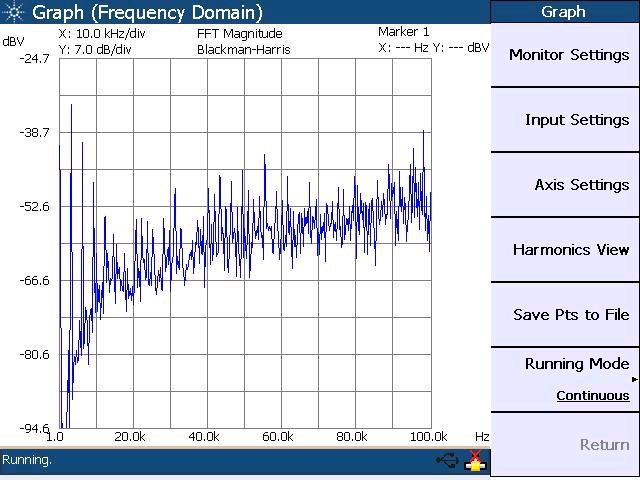
\includegraphics[scale=0.5]{../EJ4/Mediciones/0.5Gauss/s2_ns.jpeg}
\par\end{centering}
\caption{Visualización de efecto de noise shaping en la señal digital}
\end{figure}

En este caso, la salida digital para la señal 1/2 Gauss presenta un espectro donde el efecto de noise shaping resulta más visible que en el caso senoidal. También, por otra parte, se observa la parte del espectro en banda base que pasó por el filtro antialias (que no es el espectro completo, por lo explicado sobre el ancho de banda de la señal en cuestión previamente).

\newpage

A modo de prueba, se disminuyó una década la frecuencia de la señal gaussiana (es decir a 300Hz), para que pasen más armónicos a través del filtro antialias y poder observar una salida recuperada más fiel a la entrada. Las señales resultantes se muestran a continuación.

\begin{figure}[!ht]
\begin{centering}
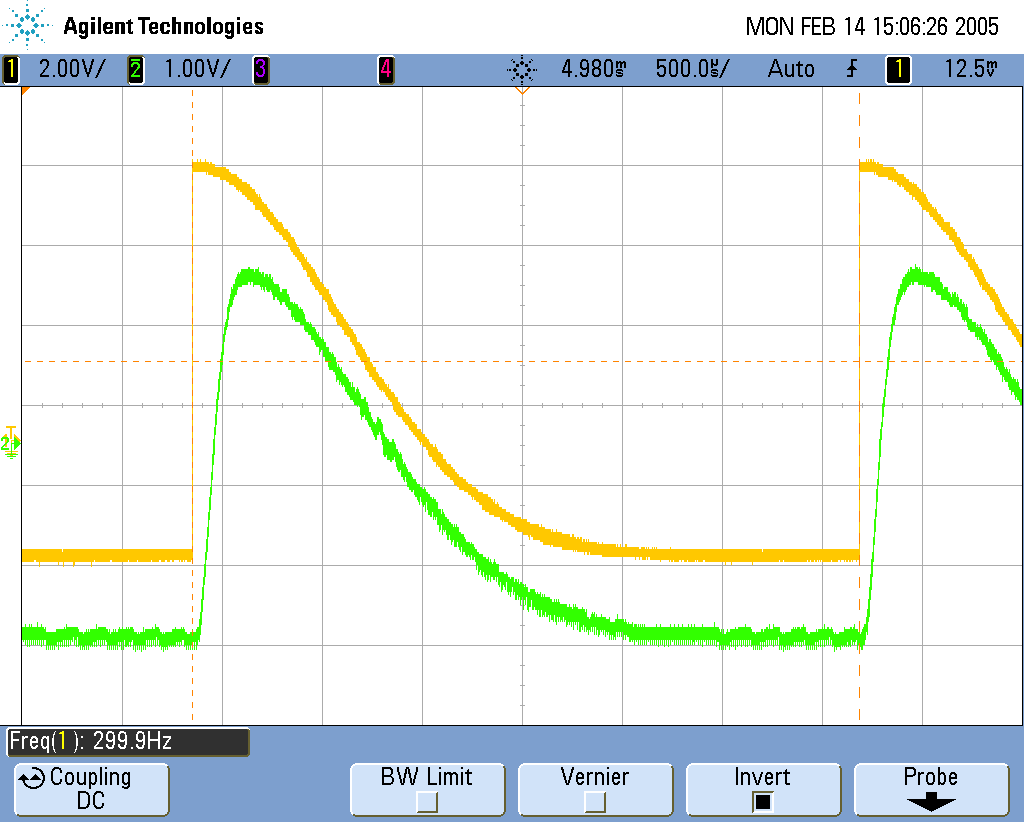
\includegraphics[scale=0.25]{../EJ4/Mediciones/example.png}
\par\end{centering}
\caption{Señal de entrada y recuperada - Atenuación (CH1: Entrada, CH2: Salida) - Ejemplo a 300Hz}
\end{figure}

\subsubsection{Sinc}

Para esta señal, considerando que se pedía una frecuencia mínima de 3.3KHz, se utilizó una cercana (4KHz). De esta forma, siendo el espectro de la sinc un pulso rectangular entre [-4KHz 4 KHz], se logra conservar todo el espectro al pasar por el filtro antialias, dado que la frecuencia de corte se encontraba en 6KHz.

\begin{figure}[!ht]
\begin{centering}
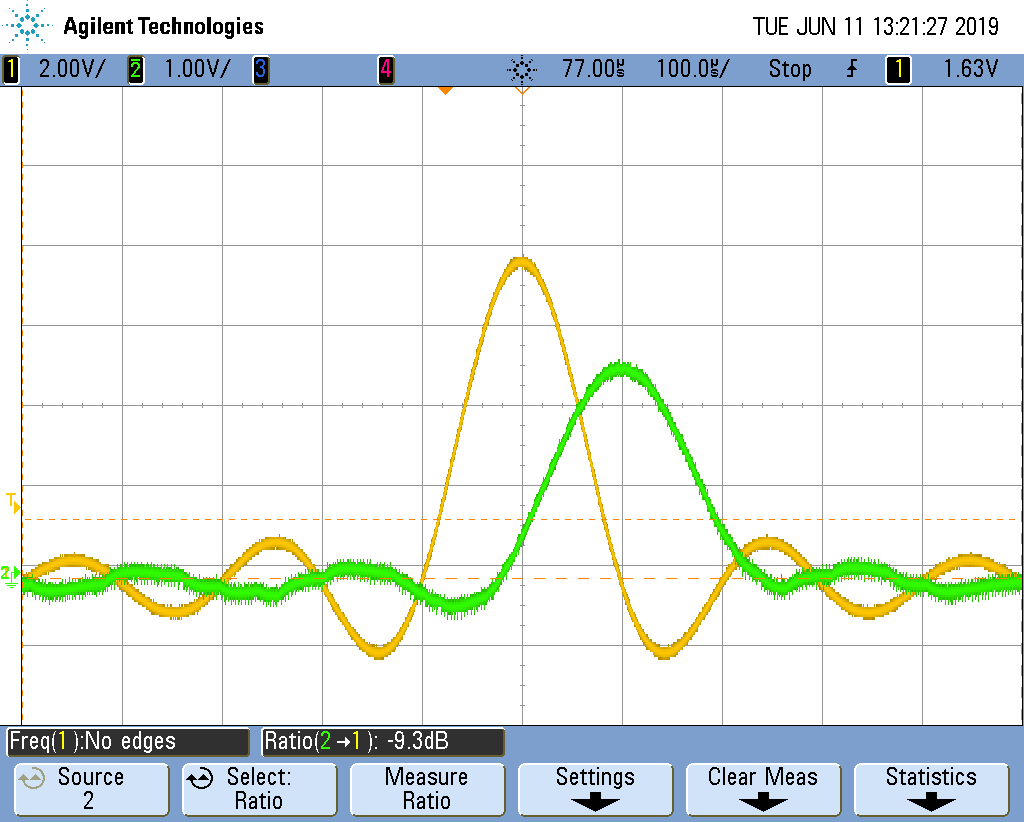
\includegraphics[scale=0.25]{../EJ4/Mediciones/Sinc/s3_1a.png}
\par\end{centering}
\caption{Señal de entrada y recuperada - Atenuación (CH1: Entrada, CH2: Salida)}
\end{figure}

Siguiendo el mismo criterio que para la señal 1/2 Gauss, el factor de oversampleo L = 64, resulta en una frecuencia de sampleo de aproximadamente 600KHz, por lo que se configuró el oscilador a dicha frecuencia. Como se esperaba, a la salida se obtiene una buena representación de la señal de entrada, dado que el espectro de ésta es acotado (como se mencionó previamente).

\newpage

\begin{figure}[!ht]
\begin{centering}
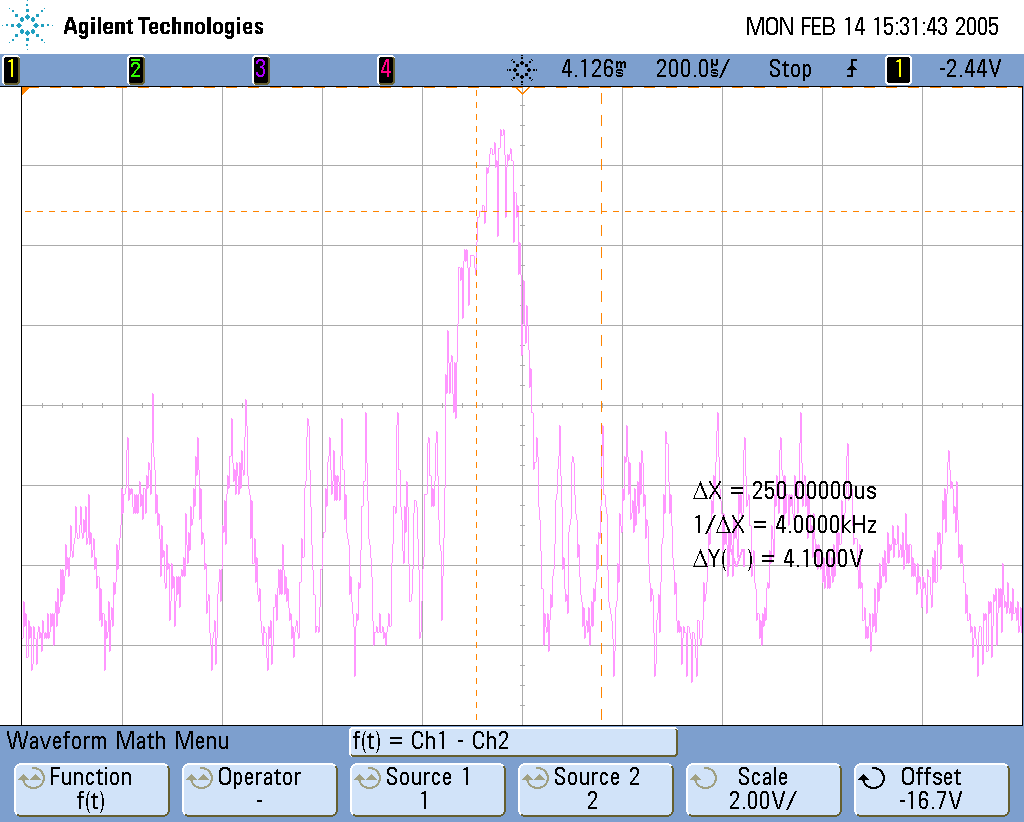
\includegraphics[scale=0.25]{../EJ4/Mediciones/Sinc/dif_sinc.png}
\par\end{centering}
\caption{Señal de entrada y salida diferencial - (CH1: Entrada, CH2: Salida diferencial)}
\end{figure}

La señal diferencial medida a la salida del integrador mediante el mismo método que en los casos anteriores resulta, como era de esperar, que siguiera la forma de la Sinc original, sumado a la respuesta a la señal cuadrada proveniente del DAC.


\begin{figure}[!ht]
\begin{centering}
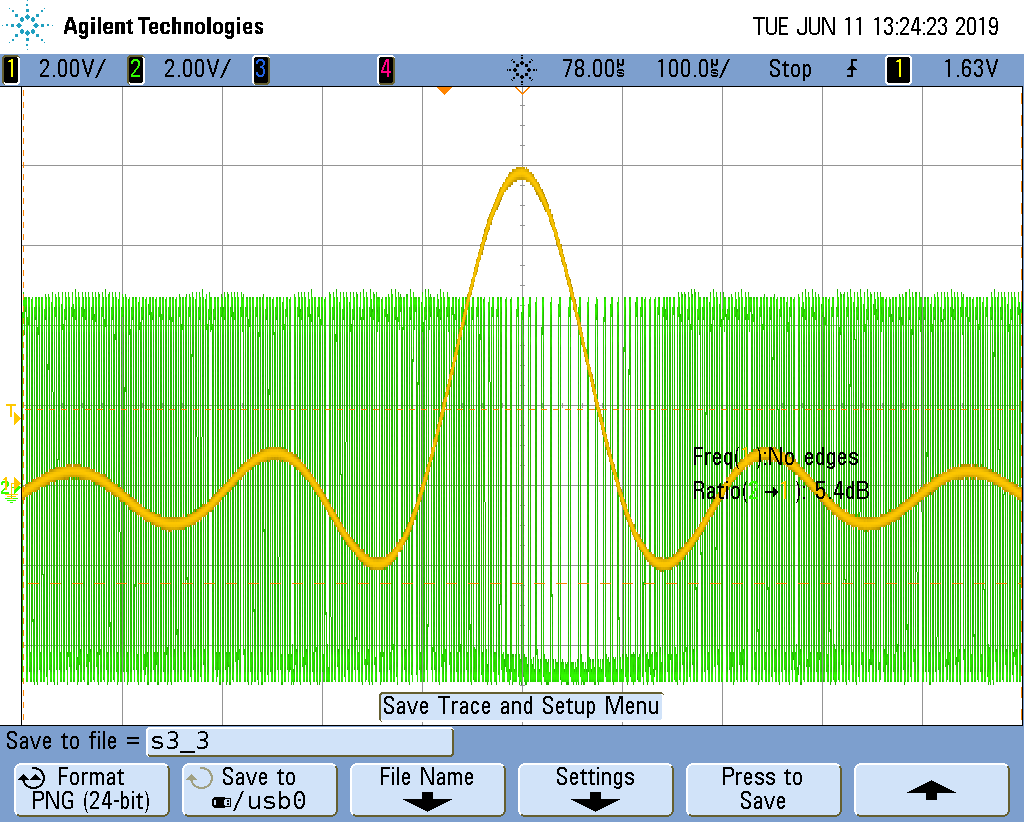
\includegraphics[scale=0.25]{../EJ4/Mediciones/Sinc/s3_3.png}
\par\end{centering}
\caption{Señal de entrada y salida digital - (CH1: Entrada, CH2: Salida digital)}
\end{figure}

En la figura, se observa la señal digital resultante, con características similares a las explicadas para las dos señales de prueba anteriores.

\newpage

\begin{figure}[!ht]
\begin{centering}
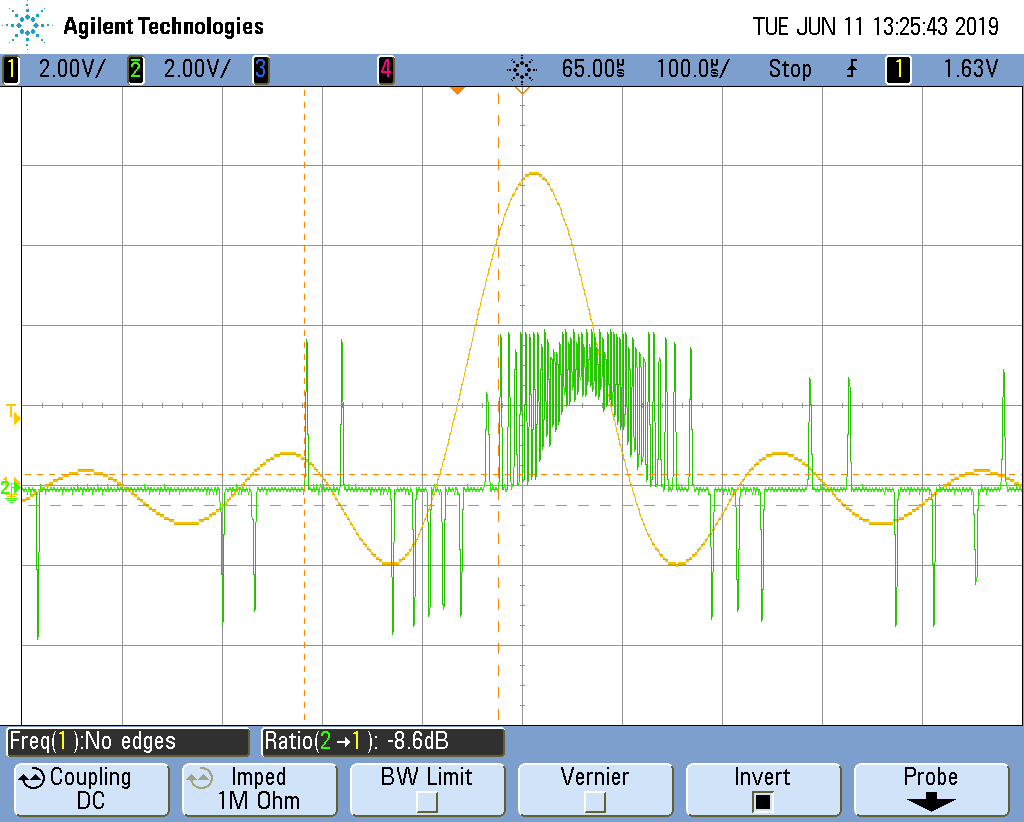
\includegraphics[scale=0.25]{../EJ4/Mediciones/Sinc/s3_4.png}
\par\end{centering}
\caption{Señal de entrada y salida digital - (CH1: Entrada, CH2: Salida digital con average máximo)}
\end{figure}

En este último caso, se realizó también la promediación la señal digital con el osciloscopio. El lóbulo central, que es el de mayor amplitud es el que mejor queda respresentado por el promedio, mientras que los lóbulos laterales, al atenuarse rápidamente, en la promediación prácticamente se anulan, pero quedan remanentes algunos picos representativos en los lugares donde el seno toma su valor pico.

\begin{figure}[!ht]
\begin{centering}
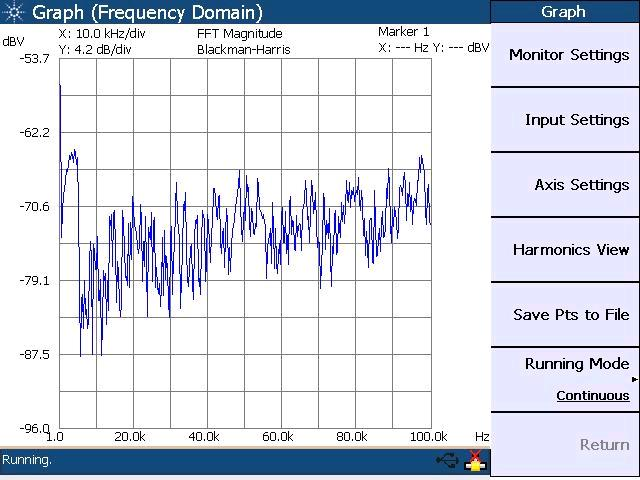
\includegraphics[scale=0.5]{../EJ4/Mediciones/Sinc/s3_ns.jpeg}
\par\end{centering}
\caption{Visualización de efecto de noise shaping en la señal digital}
\end{figure}

En este caso, la señal digital correspondiente a la Sinc posee un espectro donde no es tan notorio el efecto de noise shaping, pero de igual forma presenta la característica de que la atenuación disminuye al aumentar la frecuencia (aunque en forma leve). En banda base además se logra ver la parte del espectro de la sinc para frecuencias positivas (recordar que el espectro que le corresponde es un pulso centrado en 0 que va, en este caso, desde -4KHz a 4Khz).

\end{document}